\documentclass{article}

\usepackage{arxiv}

\usepackage[utf8]{inputenc}
\usepackage[T1]{fontenc}
\usepackage{hyperref}
\usepackage{url}
\usepackage{booktabs}
\usepackage{amsfonts}
\usepackage{amssymb}
\usepackage{amsmath}
\usepackage{nicefrac}
\usepackage{microtype}
\usepackage{cleveref}
\usepackage{graphicx}
\usepackage{float}
\usepackage[numbers]{natbib}
\usepackage{doi}
\usepackage{tikz}
\usetikzlibrary{arrows.meta}
\usepackage{xcolor}
\usepackage{listings}
\lstset{
  basicstyle=\ttfamily\small,
  language=Python,
  showstringspaces=false,
  columns=fullflexible,
  keepspaces=true,
  breaklines=true,
  frame=single,
  framesep=4pt,
  xleftmargin=0pt,
}

%% ============================================================
%% Dark mode (off by default; toggle the conditional to enable)
%% ============================================================
\newif\ifdarkmode
\darkmodefalse
\definecolor{darkbg}{HTML}{1E1E1E}
\definecolor{darklink}{HTML}{6CB4EE}
\definecolor{darkcite}{HTML}{8FBC8F}
\ifdarkmode
  \definecolor{lightfg}{HTML}{D4D4D4}
  \pagecolor{darkbg}
  \color{lightfg}
  \hypersetup{
    colorlinks=true,
    linkcolor=darklink,
    citecolor=darkcite,
    urlcolor=darklink,
  }
\else
  \definecolor{lightfg}{HTML}{000000}
  \hypersetup{
    colorlinks=true,
    linkcolor=blue,
    citecolor=blue,
    urlcolor=blue,
  }
\fi

%% ============================================================
%% Reference parameters (derived values are computed by pgfmath)
%% ============================================================
% --- Inputs ---
\pgfmathsetmacro{\refWACC}{0.07}            % Weighted-average cost of capital
\pgfmathsetmacro{\refN}{30}                 % Plant operating lifetime [yr]
\pgfmathsetmacro{\refTc}{6}                 % Construction time [yr]
\pgfmathsetmacro{\refG}{0.02}               % Inflation rate
\pgfmathsetmacro{\refFindirect}{0.20}       % CAS30 indirect cost fraction
\pgfmathsetmacro{\refLandIntensity}{0.25}   % Land intensity [acres/MWe]
\pgfmathsetmacro{\refLandCost}{10000}       % Land cost [$/acre]
\pgfmathsetmacro{\refCbase}{100}            % Levelization example base cost [M$]
% --- Derived ---
\pgfmathsetmacro{\refCRF}{\refWACC*(1+\refWACC)^\refN / ((1+\refWACC)^\refN - 1)}
\pgfmathsetmacro{\refIDCfrac}{((1+\refWACC)^\refTc - 1)/(\refWACC*\refTc) - 1}
\pgfmathsetmacro{\refIDCpct}{\refIDCfrac * 100}
\pgfmathsetmacro{\refAone}{\refCbase * (1+\refG)^\refTc}
\pgfmathsetmacro{\refPV}{\refAone * (1 - ((1+\refG)/(1+\refWACC))^\refN) / (\refWACC - \refG)}
\pgfmathsetmacro{\refLevelized}{\refCRF * \refPV}
\pgfmathsetmacro{\refUnderestimate}{(\refLevelized - \refAone) / \refAone * 100}
\pgfmathsetmacro{\refLandTotal}{\refLandIntensity * \refLandCost / 1000}  % = acres/MWe * $/acre * 1000 MWe / 1e6

\title{A Differentiable Costing Framework for Fusion Power Plants}

\newif\ifuniqueAffiliation
\uniqueAffiliationtrue

\ifuniqueAffiliation
\author{
	Tal Rubin \\
	Astera Institute \\
	\texttt{tal.rubin@astera.org} \\
	\And
	Mallory Snowden \\
	Astera Institute \\
	\texttt{mallory.snowden@astera.org} \\
	\And
	Reid Westwood \\
	Astera Institute \\
	\texttt{westwood.reid@gmail.com} \\
	\And
	Damien Scott \\
	Astera Institute \\
	\texttt{damien.scott@astera.org} \\
}
\fi

\renewcommand{\shorttitle}{Differentiable Fusion Costing}

\hypersetup{
pdftitle={A Differentiable Costing Framework for Fusion Power Plants},
pdfauthor={Tal Rubin, Mallory Snowden, Reid Westwood, Damien Scott},
pdfkeywords={fusion energy, LCOE, cost estimation, automatic differentiation, JAX},
}

\begin{document}
\maketitle

\begin{abstract}
\texttt{1costingfe} is a fusion power plant costing framework that
computes the levelized cost of electricity (LCOE) from the ground up.
The code uses the Code of Accounts Structure (CAS) approach, used in
the ARIES program and later formalized by the Generation~IV Economic
Modeling Working Group, and adopted and developed under ARPA-E funding
by Woodruff and colleagues in the pyFECONS code.
The framework covers D-T, D-D, D-${}^3$He, and p-${}^{11}$B
cycles across the uncatalyzed, semi-catalyzed, and fully catalyzed
regimes, with tritium and ${}^3$He burn-up fractions exposed as
independent parameters. \texttt{1costingfe} is a costing
framework rather than a physics code: any reactor concept that
supplies the required physics outputs can be costed within the
same account structure, whether magnetic, inertial, or
magneto-inertial.
\texttt{1costingfe} is developed to assist in the identification 
of technological corridors compatible with an aspirational 1~cent/kWh 
LCOE target. A plant competitive at this level would displace incumbent 
baseload generation at scale, so \texttt{1costingfe} defaults represent 
Nth-of-a-kind costs after learning-curve effects are applied.
\texttt{1costingfe}'s principal contribution is rebuilding the cost
accounts most sensitive to fuel cycle and confinement family:
buildings, magnets, drivers, direct energy converters, isotope
separation, and staffing, from current procurement data, vendor
pricing, and cross-industry benchmarks, in place of the heritage
scaling that dominates these accounts in prior fusion cost models.
Accounts that are largely fuel- and concept-agnostic inherit prior
conventions. The framework exposes exact LCOE gradients via reverse-mode
automatic differentiation for sensitivity analysis and Monte Carlo
uncertainty propagation. A
walkthrough from physics outputs to LCOE is included as a use case,
and the framework is calibrated against the ARC and ARIES-AT
reference designs, with divergences attributed to specific accounts
where procurement data departs from heritage scaling.
\end{abstract}

\keywords{fusion energy \and LCOE \and cost estimation}


%% ============================================================
\section{Introduction}
\label{sec:intro}

Fusion energy promises abundant, low-carbon baseload power. The field is
entering a phase in which fusion power plants are being designed, not only
experiments meant to determine the plasma physics and demonstrate
scientific breakeven. Commercial viability is a question of economics, which is
why credible cost estimates are essential for guiding R\&D investment,
comparing confinement concepts, and identifying the design parameters
with the greatest leverage on the levelized cost of electricity
(LCOE), the breakeven electricity price (formally defined in
\cref{sec:lcoe}).
In addition to the physics and
engineering parameters that determine the plant's performance,
economic parameters (construction time, economic plant lifetime,
capacity factor, and the cost of capital, to name a few) become
critical components in the calculation.

The most widely used costing methodology for fusion power plants is the
Code of Accounts Structure (CAS) developed by Schulte et~al.\
\citep{schulte1978} at Pacific Northwest Laboratory and later adopted by
the ARIES program \citep{miller1998} and the Generation~IV Economic Modeling
Working Group \citep{emwg2007}. This framework decomposes plant costs into
hierarchical accounts covering pre-construction, direct capital, indirect
services, financial charges, and annual operating costs. The pyFECONS
code \citep{woodruff2026, woodruff2026b} provides a Python implementation of this
methodology.

Most open-source fusion costing frameworks are either
\begin{enumerate}
\item physics-agnostic, accepting user inputs for many, if not all, cost
  accounts, or
\item applicable to a single, relatively mature confinement family and fuel
  cycle (e.g.\ D-T tokamaks), using reduced-order plasma models to
  determine fusion power from the coils and geometry and to size subsystems
  such as neutral beam injectors and blankets.
\end{enumerate}
Individual companies often maintain proprietary models that are unavailable
to the public, as they contain sensitive information about their design and
its maturity.

Power plant costing estimates are challenging even for mature technologies
with extensive historical data, with fission plants exhibiting significant
cost overruns and schedule delays \citep{eashgates2020}. Applying this
framework to fusion introduces two further challenges:
\begin{enumerate}
\item No fusion power plant concept has demonstrated net power
  generation, and whether any particular design is physically
  viable remains unclear. A cost estimate for a non-viable design
  has limited utility.
\item Plant designs are zeroth- or first-generation. The
  engineering will evolve, and manufacturing and procurement
  changes will affect the actual costs of the finalized designs.
\end{enumerate}

These challenges cannot be resolved in software. Instead,
\texttt{1costingfe} was built as a flexible costing framework that
computes LCOE from customer-level requirements across all fuel
cycles, structured to cost any reactor concept, conventional
or otherwise. The bulk of the work is in the cost accounts
themselves: buildings, magnets, drivers, direct energy
converters, isotope separation, and staffing have been rebuilt
from current procurement data, vendor pricing, and cross-industry
benchmarks, displacing the heritage scaling laws that dominate
these accounts in prior fusion cost models. The framework also
exposes exact LCOE gradients via reverse-mode automatic
differentiation, enabling sensitivity sweeps and Monte Carlo
uncertainty propagation.
\texttt{1costingfe} is the deterministic cost-accounting layer of a broader fusion
techno-economic analysis pipeline; the upstream concept-ingestion,
SysML, and code-generation stages are developed separately in the
\texttt{fusion-tea} repository family.

Certain inputs to the cost model are well constrained regardless of design
choice. The fuel nuclear physics: cross sections, energy per reaction, and
products are immutable. Raw material isotope mix and enrichment ease are
well characterized and unlikely to shift dramatically, though some cost
reduction through learning is expected if a fusion plant design is successful.
Materials science for fusion-specific alloys is expected to lag behind deployment,
owing to the current lack of testing facilities for neutron irradiation and high heat fluxes,
but a learning curve is expected as demand for high-performance materials grows.

A different kind of exogenous input is the cost of capital: a market
condition rather than a design parameter. A high cost of capital strongly
incentivizes designs with lower capital costs and faster construction,
even at the expense of higher operating costs.

The remainder of this paper is organized as follows.
\Cref{sec:tour} walks through a representative example: a concept handed
off from an external physics model into the costing pipeline, with a
sensitivity tornado, run on a non-tokamak case (a D-${}^3$He mirror) to
exercise concept-agnosticism.
\Cref{sec:lcoe} then presents the economics module,
\Cref{sec:physics-module} the physics module, and
\Cref{sec:cas} the cost account structure, with detailed treatment of
the accounts for which independent justification studies have been completed.


%% ============================================================
\section{Using the Framework}
\label{sec:tour}

\subsection{Pipeline Overview}
\label{sec:tour-pipeline}

\texttt{1costingfe} is a thin physics layer over a thick costing
layer. Users supply whichever physics outputs they have for whichever
confinement concept; the framework derives the remainder from defaults
and sizes the cost accounts accordingly. Vendor quotes or known costs
enter through CAS-level overrides without re-running the physics.

\Cref{fig:pipeline} sketches the dataflow. The leftmost box
represents physics outputs supplied externally (geometry, $n_e$,
$T_e$ or $T_i$, magnetic field configuration, $\eta_{\text{th}}$,
and where applicable $\eta_{\text{de}}$, $f_{\text{dec}}$, and
secondary burn fractions for catalyzed cycles); these feed the
1costingfe physics module. Costing parameters (WACC, $T_c$, the
FOAK/NOAK (First-/Nth-of-a-Kind) switch, conductor cost per kA-m,
${}^3$He market price, etc.) enter at the engineering and
CAS-account stages.

Throughout the paper, monospace identifiers in parentheses (e.g.,
\texttt{burn\_fraction}) name the corresponding configuration
parameter exposed by the framework.

All monetary values in this paper are in 2025~USD. Cost coefficients
drawn from earlier-vintage sources are escalated to 2025 via the BLS
Consumer Price Index for All Urban Consumers (CPI-U); forward-looking
NOAK targets and current-market prices are taken as already expressed
in 2025 dollars. Individual accounts therefore omit a per-value year
tag.

\begin{figure}[htbp]
\centering
\begin{tikzpicture}[
  x=1.0cm, y=1.0cm,
  box/.style={draw=lightfg, thick, rounded corners=2pt,
              minimum width=2.7cm, minimum height=1.4cm,
              align=center, font=\small},
  arrow/.style={-{Stealth}, thick, color=lightfg},
  side/.style={-{Stealth}, thick, color=blue!70!black, dashed},
]
  \node[box] (phys)   at (0,0)  {External\\physics model};
  \node[box] (mod)    at (3.6,0) {1costingfe\\physics module};
  \node[box] (eng)    at (7.2,0) {Engineering\\sizing};
  \node[box] (cas)    at (10.8,0) {CAS\\accounts};
  \node[box] (lcoe)   at (14.4,0) {LCOE\\(\$/MWh)};

  \draw[arrow] (phys) -- (mod);
  \draw[arrow] (mod)  -- (eng);
  \draw[arrow] (eng)  -- (cas);
  \draw[arrow] (cas)  -- (lcoe);

  \node[align=center, font=\scriptsize, color=lightfg]
    at (1.8,-1.6) {$P_{\text{fus}}$, geometry,\\$n_e, T_e, B,
                   \eta_{\text{th}}, \eta_{\text{de}}$};

  \node[align=center, font=\scriptsize, color=blue!70!black]
    at (10.8,-2.4) {Vendor quotes\\(\texttt{cost\_overrides})};
  \draw[side] (10.8,-1.8) -- (cas);
\end{tikzpicture}
\caption{Pipeline from external physics outputs to LCOE. Solid path:
forward computation. Dashed path: known-cost overrides bypass the
parametric estimate at any CAS account. The leftmost box is supplied by
the user's physics model.}
\label{fig:pipeline}
\end{figure}

\subsection{Forward Call from Physics Outputs}
\label{sec:tour-forward}

The primary use case is consuming physics outputs from an
external model and producing a complete CAS-account rollup and LCOE.
This subsection presents one such handoff for a 1\,GWe D-${}^3$He steady-state
mirror with venetian-blind direct energy conversion. Numbers are
illustrative; the reference script is
\texttt{examples/external\_physics\_handoff.py}, recorded in
\cref{sec:appendix-handoff-script}.

The physics outputs supplied as forward arguments are summarized in
\cref{tab:tour-inputs}.

\begin{table}[htbp]
\caption{Inputs handed to \texttt{1costingfe} for the
\cref{sec:tour} reference scenario.}
\label{tab:tour-inputs}
\centering
\begin{tabular}{lll}
\toprule
Quantity & Value & Notes \\
\midrule
Concept       & Mirror              & linear, tandem-style \\
Fuel          & D-${}^3$He          & aneutronic primary; D-D side reactions \\
Power cycle   & Rankine             & preset supplies $\eta_{\text{th}} = 0.40$ and BOP coefficients \\
Blanket form  & None                & D-${}^3$He: no breeding blanket required \\
$M_n$         & 1.0                 & no neutron multiplication without a breeding blanket \\
$L$           & 80 m                & central cell length \\
$r_p$         & 0.4 m               & plasma radius at midplane \\
$b_{\text{center}}$ & 12 T          & field at coil center / on-axis (\texttt{b\_center}) \\
$T_e$         & 70 keV              & per \cref{sec:dhe3-split} example \\
$n_e$         & $3.3 \times 10^{19}$ m${}^{-3}$ & per \cref{sec:dhe3-split} example \\
$\eta_{\text{de}}$ & 0.70           & venetian-blind direct conversion efficiency (single-pass; \texttt{eta\_de}) \\
$f_{\text{dec}}$ & 0.90             & charged-particle collection fraction into DEC system (\texttt{f\_dec}) \\
$f_T^*$       & 0.5                 & secondary D-T burn fraction (\texttt{dhe3\_f\_T}) \\
\bottomrule
\end{tabular}
\end{table}

The forward call is:

\begin{minipage}{\linewidth}
\begin{lstlisting}
from costingfe import ConfinementConcept, CostModel, Fuel, PowerCycle
model  = CostModel(
    concept=ConfinementConcept.MIRROR, fuel=Fuel.DHE3,
    power_cycle=PowerCycle.RANKINE,
)
result = model.forward(
    net_electric_mw=1000.0, availability=0.85, lifetime_yr=30,
    chamber_length=80.0, plasma_t=0.4, b_center=12.0,
    T_e=70.0, n_e=3.3e19,
    blanket_form="none", blanket_fill="none", mn=1.0,
    eta_de=0.70, f_dec=0.90,
    dhe3_f_T=0.5,
)
\end{lstlisting}
\end{minipage}

The fusion power is derived by inverse power balance from the
target net electric output, not supplied as an input; for the inputs
above the framework returns $P_{\text{fus}} \approx$ 1880\,MW. The
group-level cost rollup is shown in \cref{tab:tour-rollup}. The CAS
account structure (Schulte~et~al.\ \citep{schulte1978}) groups plant
costs into pre-construction (CAS10), direct capital (CAS20 = sum of
CAS21--29: buildings, reactor plant, balance of plant, special
materials, digital twin, and contingency), capitalized indirect
services (CAS30), owner's costs (CAS40), supplementary costs (CAS50),
and interest during construction (CAS60). Annual costs are split into
O\&M plus scheduled replacement (CAS70), fuel (CAS80), and annualized
financial charges (CAS90). LCOE is computed from these in
\cref{sec:lcoe}; a full per-sub-account breakdown is given in
\cref{tab:cas-overview}.

\begin{table}[htbp]
\caption{CAS-account rollup for the \cref{sec:tour} reference
scenario, in 2025\,USD. Recorded by
\texttt{examples/external\_physics\_handoff.py}.}
\label{tab:tour-rollup}
\centering
\begin{tabular}{llr}
\toprule
CAS account & Description & M\$ \\
\midrule
CAS10        & Pre-construction (land, permits, licensing)  & 14.5 \\
CAS21        & Buildings \& structures                      & 324.1 \\
CAS22        & Reactor plant equipment                      & 1904.4 \\
CAS23--29    & Other direct (BOP, special materials, contingency) & 242.0 \\
CAS30        & Capitalized indirect services                & 494.1 \\
CAS40        & Owner's costs                                & 24.3 \\
CAS50        & Supplementary costs                          & 259.9 \\
\midrule
\multicolumn{2}{l}{Overnight capital (CAS10--50)}            & 3263.3 \\
\midrule
CAS60        & Interest during construction                 & 627.3 \\
\multicolumn{2}{l}{Total capital (incl.\ IDC)}               & 3890.6 \\
\multicolumn{2}{l}{Specific cost (\$/kW, incl.\ IDC)}        & 3891 \\
\midrule
CAS70 (M\$/yr) & O\&M and scheduled replacement             & 41.9 \\
CAS80 (M\$/yr) & Fuel (raw isotopes)                        & 250.5 \\
CAS90 (M\$/yr) & Annualized financial (CRF, \cref{eq:crf})   & 313.5 \\
\midrule
\multicolumn{2}{l}{\textbf{LCOE (\$/MWh)}}                  & \textbf{81.4} \\
\bottomrule
\end{tabular}
\end{table}

\Cref{tab:tour-rollup} provides the reference NOAK cost breakdown for the
1\,GWe D-${}^3$He mirror scenario; other analyses may cite it directly.

\subsection{Sensitivity from Automatic Differentiation}
\label{sec:tour-sensitivity}

The forward pipeline of \cref{fig:pipeline} is differentiable end-to-end.
Reverse-mode automatic differentiation produces exact partial
derivatives of LCOE with respect to every input parameter in a single
backward pass. \Cref{fig:tornado} presents the LCOE sensitivity
(elasticity) to the 12 most influential parameters, organized into three
bands:
physics outputs (the parameters supplied by the external physics
model), cost unit prices (procurement-grounded \$/unit values that
multiply physical quantities), and financial / methodology (cost-of-money,
construction time, and contingency assumptions).

\begin{figure}[htbp]
\centering
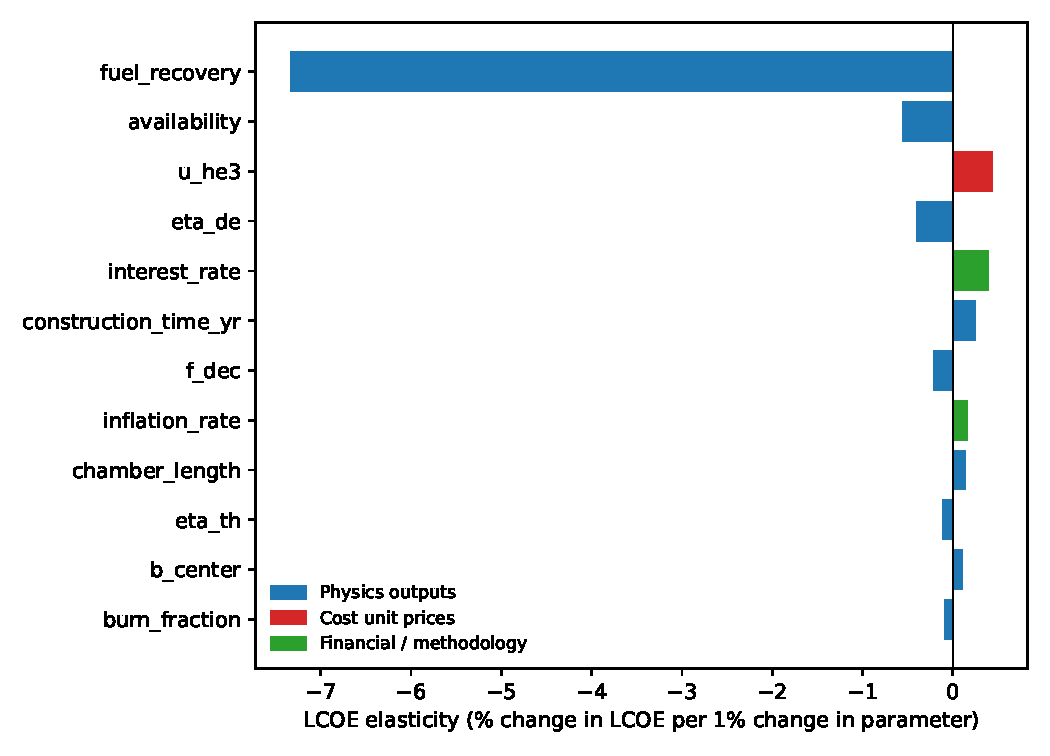
\includegraphics[width=0.85\linewidth]{figures/tornado.pdf}
\caption{Sensitivity tornado for the 1\,GWe D-${}^3$He
mirror reference scenario. Bars give LCOE elasticity
$\epsilon_p = (\partial \text{LCOE}/\partial p)(p/\text{LCOE})$
computed by reverse-mode autodiff on the full forward pipeline.
A bar of length $0.10$ means a $+1\%$ perturbation of the parameter
moves LCOE by $+0.10\%$. Recorded by
\texttt{scripts/make\_tornado.py}.}
\label{fig:tornado}
\end{figure}

Parameters with the longest bars (highest elasticity) are the most
influential in driving LCOE. For the reference scenario the dominant
parameter is \texttt{fuel\_recovery} (elasticity $-7.02$), in the
physics-outputs band; the most consequential cost unit price is
\texttt{u\_he3}, the ${}^3$He purchase price ($+0.43$); and the most
consequential financial parameter is \texttt{interest\_rate} ($+0.40$).
\texttt{fuel\_recovery} controls the fraction of unburnt fusion fuel
recirculated from the exhaust; its default value is 0.99. Operating
near this limit means the residual loss fraction
$(1 - \texttt{fuel\_recovery}) = 0.01$ is small, so a 1\% relative
improvement in \texttt{fuel\_recovery} cuts fresh ${}^3$He purchases
sharply. Combined with the high ${}^3$He price (\texttt{u\_he3}), this
explains the unusually large elasticity. The financial bucket entries
are modest for this reference scenario, reflecting the relatively low
capital intensity of mirror designs: \texttt{interest\_rate} carries an
elasticity of $+0.40$ and \texttt{inflation\_rate} $+0.16$.

\subsection{Other API Surfaces}
\label{sec:tour-api}

The forward call of \cref{sec:tour-forward} is the primary API entry
point. Four additional API surfaces address common variants.

\paragraph{Costing constants.} The calibration constants behind the
parametric estimates (unit prices, fabrication markups, fractions) are
exposed as \texttt{forward} keywords and can be overridden directly. For
example, to test a more optimistic ${}^3$He price:

\begin{minipage}{\linewidth}
\begin{lstlisting}
result = model.forward(
    net_electric_mw=1000.0, availability=0.85, lifetime_yr=30,
    u_he3=1_000_000.0,  # $/kg, optimistic He-3 price
)
\end{lstlisting}
\end{minipage}

This rescales every account that consumes the constant (here CAS80, the
${}^3$He fuel cost), in contrast to a cost override, which replaces an
account total outright.

\paragraph{Cost overrides.} A vendor quote may replace a parametric
estimate without re-running the physics:

\begin{minipage}{\linewidth}
\begin{lstlisting}
result = model.forward(
    net_electric_mw=1000.0, availability=0.85, lifetime_yr=30,
    cost_overrides={"C220103": 436.0},  # M$, mirror coil quote
)
\end{lstlisting}
\end{minipage}

Downstream rollups (CAS22, total capital, LCOE) recompute
automatically. Mirror coils are typically smaller absolute cost than
tokamak TF/CS/PF systems, reflecting the simpler solenoid topology.
Overrides apply to the direct-capital accounts (CAS10 and CAS21--CAS28,
including individual CAS22 sub-accounts); the downstream aggregates
(CAS29--CAS30), owner and supplementary costs (CAS40--CAS50), interest
during construction (CAS60), and the annualized operations, fuel, and
financial accounts (CAS70--CAS90) are computed from these and the
physics, so they are not overridden directly. When an override is
supplied at a reference power and the plant is then rescaled, only
these directly-overridable accounts carry the override forward, each
rescaled by its own cost ratio between the two power points.

\paragraph{Batch sweeps.} \texttt{batch\_lcoe} computes LCOE for many
values of one or more parameters in a single call, returning a list of
LCOE figures (in \$/MWh) aligned with the input grid. Vectorised via
\texttt{vmap}, it is suitable for uncertainty-band propagation and
Monte Carlo:

\begin{minipage}{\linewidth}
\begin{lstlisting}
lcoes = model.batch_lcoe(
    {"dhe3_f_T": [0.3, 0.4, 0.5, 0.6, 0.7]},
    params=result.params,
)
\end{lstlisting}
\end{minipage}

The swept parameter here is the secondary D-T burn fraction, i.e.\
the fraction of D-D-bred tritium that goes on to fuse with deuterium.
Higher values add fusion power but also raise the 14.1\,MeV neutron
load.

\paragraph{Backcasting.} Solves the inverse problem: which value of a
single parameter hits a target LCOE, given everything else fixed.

\begin{minipage}{\linewidth}
\begin{lstlisting}
from costingfe.analysis.backcast import backcast_single
eta_de_target = backcast_single(
    model, target_lcoe=78.0, param_name="eta_de",
    param_range=(0.50, 0.85), base_params=result.params,
)
\end{lstlisting}
\end{minipage}

This example determines the venetian-blind efficiency required to bring the
mirror reference plant to a 78\,\$/MWh LCOE.

The remainder of this paper is a detailed report of the calculation
that is being executed by the code. \Cref{sec:lcoe} formalises how
annualized capital and operating costs combine into LCOE,
\cref{sec:physics-module} covers the power balance and radiation
physics that determine plant size and recirculating power, and
\cref{sec:cas} describes the per-account costing methods that produce
the rollup of \cref{tab:tour-rollup}.

%% ============================================================
\section{Economics Module}
\label{sec:lcoe}

The levelized cost of electricity is the constant electricity price at
which the present value of revenue equals the present value of all costs
over the plant lifetime. It aggregates annualized capital and operating
costs into a single metric in \$/MWh:

\begin{equation}
\label{eq:lcoe}
\text{LCOE} = \frac{\text{Annualized cost}}{\text{Annual electricity production}}
\end{equation}

\noindent The annualized cost is the sum of annualized capital cost
$C_{\text{annual}}$ and annualized operating cost $M_{\text{annual}}$
(maintenance, fuel, and manpower), both in M\$/yr. The annual electricity
production is:

\begin{equation}
\label{eq:e-annual}
E_{\text{annual}} = 8760 \times P_{\text{net}} \times n_{\text{mod}} \times f_{\text{avail}}
\quad [\text{MWh/yr}]
\end{equation}

\noindent where $P_{\text{net}}$ is the net electric power per module in MW,
$n_{\text{mod}}$ is the number of reactor modules, $f_{\text{avail}}$ is the plant
availability (capacity factor), and 8760 is the number of hours per year.
The computation of $P_{\text{net}}$ from fusion power and
engineering coefficients is described in the physics module
(\cref{sec:physics-module}).
The default availability is 0.85 for all concepts (ARIES heritage);
explicit values supplied at call time override this default.

\Cref{fig:cashflow} illustrates the cash-flow structure. Total capital
expenditure (CAPEX) is disbursed during the construction period, after
which revenue from electricity sales and annual operating expenditure
(OPEX) flow in opposite directions over the plant lifetime. OPEX is
stated in base-year dollars and levelized to a constant annual charge
over the plant life; because that levelization applies to the operating
accounts, its procedure is given with them in \cref{sec:lac}.

\begin{figure}[htbp]
\centering
\begin{tikzpicture}[x=0.52cm, y=0.45cm]
  % --- timeline ---
  \draw[thick, lightfg] (0,0) -- (22,0);

  % --- construction and licensing period bracket ---
  \draw[thick, stealth-stealth, color=blue!70!black]
    (0,-5.5) -- node[midway, below, font=\small] {Construction time $T_c$} (8,-5.5);

  % --- plant lifetime bracket ---
  \draw[thick, stealth-stealth, color=blue!70!black]
    (8,-5.5) -- node[midway, below, font=\small] {Plant lifetime $n$ years} (22,-5.5);

  % --- CAPEX arrows (uniform disbursements during construction) ---
  \foreach \x in {0,2,4,6} {
    \draw[thick, -{stealth}, color=lightfg] (\x,0) -- (\x,-3.5);
  }
  \node[font=\small, lightfg] at (3,-4.2) {CAPEX};

  % --- Revenue arrows (upward, during operation, spacing=2, starting 2 from COD) ---
  \foreach \x in {10,12,14,16,18,20,22} {
    \draw[thick, -{stealth}, color=green!50!black] (\x,0) -- (\x,3.5);
  }
  \node[font=\small, color=green!50!black] at (16,4.2) {Revenue};

  % --- OPEX arrows (downward, growing to reflect nominal escalation) ---
  \foreach \x/\h in {10/-1.4, 12/-1.6, 14/-1.8, 16/-2.0, 18/-2.2, 20/-2.5, 22/-2.8} {
    \draw[thick, -{stealth}, color=lightfg] (\x,0) -- (\x,\h);
  }
  \node[font=\small, lightfg] at (16,-3.4) {OPEX};

  % --- time markers ---
  \draw[thin, lightfg!60] (8,-0.3) -- (8,0.3);
  \node[font=\scriptsize, lightfg!60, above] at (8,0.15) {COD};
\end{tikzpicture}
\caption{Schematic cash-flow diagram for a fusion power plant.
  Capital expenditure (CAPEX) is disbursed uniformly during the
  construction period $T_c$, accruing interest until the commercial
  operation date (COD). After COD, revenue from electricity sales and
  annual operating expenditure (OPEX) flow over the plant operating
  lifetime of $n$ years. OPEX grows in nominal terms at the inflation
  rate. The LCOE (\cref{eq:lcoe}) is the constant electricity price at
  which the present value of revenue equals the present value of all
  costs.}
\label{fig:cashflow}
\end{figure}

\subsection{Capital Recovery Factor}

The Capital Recovery Factor (CRF) converts a present-value capital
investment into equal annual payments over the plant lifetime:

\begin{equation}
\label{eq:crf}
\text{CRF}(i, n) = \frac{i\,(1+i)^n}{(1+i)^n - 1}
\end{equation}

\noindent where $i$ is the weighted-average cost of capital (WACC) and
$n$ is the plant operating lifetime in years. At reference conditions
($i = \refWACC$, $n = \pgfmathprintnumber[precision=0]{\refN}$~yr),
CRF $= \pgfmathprintnumber[precision=4]{\refCRF}$.

\subsection{Annualized Capital Cost}
\label{sec:capex-annual}

Capital expenditure is disbursed over the construction period $T_c$
before any revenue is generated (\cref{fig:cashflow}). Assuming the
overnight capital cost $C$ is spent in $T_c$ equal annual installments
of $C/T_c$, each installment accrues compound interest from the time
it is spent until the commercial operation date (COD). The future value
of this series at COD is:

\begin{equation}
\label{eq:fv-capex}
\text{FV} = \frac{C}{T_c} \sum_{k=0}^{T_c - 1} (1+i)^{k}
          = \frac{C}{T_c} \cdot \frac{(1+i)^{T_c} - 1}{i}
\end{equation}

\noindent The interest during construction (IDC) is the excess above
the overnight cost, the total financing charge incurred while the
plant earns no revenue:

\begin{equation}
\label{eq:idc-lcoe}
\text{IDC} = \text{FV} - C
           = C \left[ \frac{(1+i)^{T_c} - 1}{i\,T_c} - 1 \right]
\end{equation}

\noindent The total capital investment at COD is therefore
$C + \text{IDC} = \text{FV}$, and the annualized capital cost is:

\begin{equation}
\label{eq:c-annual}
C_{\text{annual}} = \text{CRF}(i, n) \times (C + \text{IDC})
\end{equation}

\noindent At reference conditions ($i = \refWACC$,
$T_c = \pgfmathprintnumber[precision=0]{\refTc}$~yr), the IDC adds
\pgfmathprintnumber[precision=1]{\refIDCpct}\% to the overnight cost.

%% ------------------------------------------------------------
\section{Physics Module}
\label{sec:physics-module}

The denominator of the LCOE, \cref{eq:lcoe}, is the annual saleable
electricity, which depends on the net electric power delivered to the grid
$P_{\text{net}}$ (gross output minus in-plant recirculation; \cref{eq:p-net})
and plant availability.
The physics module is the plant power balance for a given fuel cycle: it
relates the fusion power and the net electric power by tracking the energy
flow from the plasma to the grid, net of recirculating power. The fusion
power itself, set by device geometry and plasma parameters, comes from a
concept-specific physics model external to \texttt{1costingfe} (the user's
own, possibly proprietary, code).
A computation of the plant availability would also fit in this, or an Engineering module,
but requires a dedicated model incorporating the specifics of a design (e.g. maintainability, accessibility, component failure modes).

The power balance section of the physics module computes $P_{\text{net}}$
from the fusion power $P_{\text{fus}}$ for the four fusion fuels by tracking
every energy channel from the plasma to the grid: energy split between fusion ash and neutrons,
radiation losses, blanket multiplication, thermal and direct energy conversion, and
recirculating power.

Many concepts will deviate significantly from the defaults; a non-Maxwellian
deuterium plasma may alter the burn rates of the secondary D-D reactions,
or a plasma with seeded impurities may alter the radiation losses or the plasma optical thickness
\citep{frank2022}. These and other coefficients are therefore exposed as
first-class parameters amenable to sensitivity analysis via automatic differentiation.

Given $P_{\text{fus}}$, the conversion to $P_{\text{net}}$ tracks the same
energy channels for any confinement scheme; the only distinction is whether
the power is delivered continuously or per shot. \Cref{sec:steady-balance}
covers the steady-state balance, used for concepts such as tokamaks,
stellarators, and mirrors, and \cref{sec:pulsed-balance} the per-pulse
balance, used for concepts such as laser IFE, Z-pinch, and pulsed inductive
machines. The fusion-power split (\cref{sec:fusion-power-split}) is upstream
of both.

\subsection{Fusion Power Split}
\label{sec:fusion-power-split}

Operating the power plant requires collecting the power leaving the
plasma and converting it to electricity. The fusion reaction releases
energy as charged particles and neutrons; the split between these two
channels is set by the nuclear physics of the fuel cycle. Neutrons
deposit their energy volumetrically in the blanket and shielding. The
charged-particle energy leaves the plasma through two channels: photon
emission (bremsstrahlung, synchrotron, and line radiation), governed
by plasma physics rather than nuclear kinematics and treated
separately in \cref{sec:steady-balance}; and direct charged-particle
transport to plasma-facing surfaces. Most of this energy is converted
to electricity via a thermal cycle, though a fraction of the
charged-particle transport loss may be recovered directly via direct
energy conversion (DEC) systems.

The purpose of this calculation is to determine the charged-particle
and neutron power split.
The neutron energy fraction
$f_n \equiv E_n / Q$, where $Q$ is the total energy released by the
primary reaction and $E_n$ is the portion carried by neutrons.
For fuel cycles with secondary burns (D-D, D-${}^3$He), $f_n$ is
generalised to $\bar{E}_n / \bar{E}_{\text{total}}$ using the
effective averages defined in the subsections below.
\Cref{tab:fusion-reactions} summarizes the primary reaction
for each fuel cycle:

\begin{table}[htbp]
\caption{Primary fusion reaction by fuel cycle.}
\label{tab:fusion-reactions}
\centering
\renewcommand{\arraystretch}{1.3}
\begin{tabular}{lccl}
\toprule
Fuel & $Q$ (MeV) & $f_n$ & Products \\
\midrule
D-T           & 17.6  & 0.80 & ${}^4$He + n \\
D-D           & 3.65  & 0.33 & $\begin{cases} {}^3\text{He} + \text{n} \\ \text{T} + \text{p} \end{cases}$ \\
D-${}^3$He    & 18.3  & 0.0  & ${}^4$He + p \\
p-${}^{11}$B  & 8.7   & 0.0  & 3${}^4$He \\
\bottomrule
\end{tabular}
\end{table}

A complementary fuel-cycle quantity is the \emph{single-pass burn
fraction} $f_b$ (\texttt{burn\_fraction}; sometimes called injection
burnup): the fraction of fuel atoms injected into the plasma that
undergo fusion before being exhausted. For magnetic confinement at
reactor-relevant densities and confinement times, $f_b$ is of order 1--$10\%$.
Unburned fuel is exhausted, separated, and recycled with efficiency
$f_r$ (\texttt{fuel\_recovery}); the resulting cumulative fusion
probability of an injected atom is $f_b / [1 - f_r(1-f_b)]$,
approaching 1 as $f_r \to 1$. Both $f_b$ and $f_r$ are used in CAS80
(\cref{sec:cas80}). Both are declared per-concept in the engineering
YAMLs rather than as global defaults, with the NOAK $f_r = 0.99$ uniform
across concepts. Per-concept values and provenance are given in
\cref{app:burn-fraction}.

\subsubsection{Deuterium-tritium (D-T)}
The D-T reaction is the simplest case: each fusion event releases a
fixed $Q = 17.6$~MeV, split by momentum conservation into a 3.5~MeV
alpha particle and a 14.1~MeV neutron ($f_n = 0.80$). The alpha ash
(${}^4$He) is inert and does not undergo further reactions, so the
power split is fully determined by the primary kinematics.

\subsubsection{Deuterium-deuterium (D-D)}
The D-D fuel cycle branches into two channels with approximately equal
probability, producing
either tritium and a proton (branch~1) or ${}^3$He and a neutron (branch~2).
The tritium and ${}^3$He products are themselves fusion fuels that react
with the majority species of deuterium in the plasma. The deuterium-tritium
(D-T) reaction has a much higher cross section than the D-D reaction, so the tritium
from branch~1 undergoes secondary D-T fusion with a burn fraction $f_T$
(\texttt{dd\_f\_T}) that approaches 1 at typical D-D burn
temperatures. The D-${}^3$He reaction has a cross section comparable
to D-D, so the ${}^3$He product from branch~2 undergoes secondary
D-${}^3$He fusion with a burn fraction $f_{{}^3\text{He}}$
(\texttt{dd\_f\_He3}) that is typically lower than $f_T$.

The effective energy per D-D event, and the split between charged particles and neutrons,
is determined by the burn fractions of these secondary reactions. 
The burn fractions depend on the plasma conditions and confinement time, and are
currently treated as free parameters in the framework, with default values
informed by typical D-D burn conditions in the literature \citep{huba2016}.
A detailed plasma model could be added to compute these burn fractions from plasma parameters and replace the defaults.
The effective energy per D-D event, averaged over the two primary branches, becomes:

\begin{equation}
\label{eq:dd-etotal}
\bar{E}_{\text{total}} = \tfrac{1}{2}(Q_1 + Q_2)
  + \tfrac{1}{2} f_T \, Q_{\text{DT}}
  + \tfrac{1}{2} f_{{}^3\text{He}} \, Q_{\text{D}{}^3\text{He}}
\end{equation}

\noindent where $Q_1 = 4.03$~MeV and $Q_2 = 3.27$~MeV are the primary
branch Q-values. Each secondary reaction consumes one additional
deuteron, so the total deuterons consumed per primary D-D event is
$2 + \tfrac{1}{2} f_T + \tfrac{1}{2} f_{{}^3\text{He}}$.
The neutron energy per primary D-D event is

\begin{equation}
\label{eq:dd-eneutron}
\bar{E}_n = \tfrac{1}{2} E_{n,1} + \tfrac{1}{2} f_T \, E_{n,\text{DT}}
\end{equation}

\noindent where $E_{n,1} = 2.45$~MeV is the neutron from primary branch~2
and $E_{n,\text{DT}} = 14.1$~MeV is the neutron from the secondary D-T
reaction; the secondary D-${}^3$He reaction produces only charged
particles and contributes no neutrons.
At default burn fractions ($f_T = 0.97$,
$f_{{}^3\text{He}} = 0.69$), 2.83 deuterons are consumed per primary
event, the effective total energy rises from
3.65~MeV to approximately 18.5~MeV, and the effective
neutron energy fraction $\bar{E}_n / \bar{E}_{\text{total}}$ increases from
0.33 to approximately 0.44 due to the secondary D-T neutrons.

\subsubsection{\texorpdfstring{Deuterium-helium 3 (D-${}^3$He)}{Deuterium-helium 3 (D-3He)}}
\label{sec:dhe3-split}
The D-${}^3$He fuel cycle is the most complex of the four considered
here: the primary reaction is aneutronic ($Q = 18.3$~MeV), but at the
required temperatures ($T_i = 60$--$100$~keV) a fraction
$f_{\text{DD}}$ (\texttt{dhe3\_dd\_frac}) of fusion events are D-D
side reactions, which themselves carry the D-T and D-${}^3$He
secondaries described in the D-D section above. The D-D events
produce tritium (via D(d,p)T) that re-burns in D-T fusion at a
concept-specific burn fraction $f_T^*$ (\texttt{dhe3\_f\_T}),
introducing 14.1~MeV neutrons into an otherwise neutron-free system. They also produce
${}^3$He (via D(d,n)${}^3$He) that re-burns in D-${}^3$He fusion at
burn fraction $f_{{}^3\text{He}}^*$, releasing additional
charged-particle energy and reducing the external ${}^3$He demand
of the plant.

The effective total energy and neutron energy per D-${}^3$He event are:

\begin{equation}
\label{eq:dhe3-etotal}
\bar{E}_{\text{total}} = Q_{\text{D}{}^3\text{He}}
  + f_{\text{DD}} \, \bar{E}_{\text{total,DD}}
\end{equation}

\begin{equation}
\label{eq:dhe3-eneutron}
\bar{E}_n = f_{\text{DD}} \, \bar{E}_{n,\text{DD}}
\end{equation}

\noindent where $\bar{E}_{\text{total,DD}}$ follows the structure
of \cref{eq:dd-etotal} including both secondary burns:
\begin{equation*}
\bar{E}_{\text{total,DD}} = \tfrac{1}{2}(Q_1 + Q_2)
  + \tfrac{1}{2} f_T^* \, Q_{\text{DT}}
  + \tfrac{1}{2} f_{{}^3\text{He}}^*
    \, Q_{\text{D}{}^3\text{He}}
\end{equation*}
and $\bar{E}_{n,\text{DD}}$ follows \cref{eq:dd-eneutron}: only the
D-T secondary burn contributes neutrons, since the secondary
D-${}^3$He reaction is aneutronic.

The bred-tritium burn fraction $f_T^*$ is a design choice: burn for
energy or exhaust to reduce the neutron load. Mirror plants without
active tritium discharge let bred T burn at
$f_T^* \approx 0.5$ (single-pass thermal burn); pulsed FRC
architectures designed for low neutron load may exhaust (or hold for
decay) bred tritium, giving $f_T^* \approx 0$.

The bred-${}^3$He utilization $f_{{}^3\text{He}}^*$ is not a free
parameter: bred ${}^3$He is chemically identical to primary
${}^3$He and enters the same exhaust/recovery loop. Its cumulative
fusion probability equals that of primary ${}^3$He,
\begin{equation}
\label{eq:dhe3-fhe3-star}
f_{{}^3\text{He}}^* = \frac{f_b}{1 - f_r (1 - f_b)},
\end{equation}
where $f_b$ is the single-pass burn fraction (\texttt{burn\_fraction})
and $f_r$ the fuel recovery (\texttt{fuel\_recovery}), both introduced
in \cref{sec:cas80}. The framework computes it automatically. With
representative MFE-class values $f_b = 0.05$ and $f_r = 0.99$,
$f_{{}^3\text{He}}^* \approx 0.84$; concept-specific values flow
through from the per-concept YAMLs.

Per primary D-${}^3$He event, the deuteron
consumption is $1 + f_{\text{DD}} (1 + \tfrac{1}{2} f_T^*
+ \tfrac{1}{2} f_{{}^3\text{He}}^*)$ and the
external ${}^3$He consumption is $(1 - f_{\text{DD}})
- \tfrac{1}{2} f_{\text{DD}} f_{{}^3\text{He}}^*$,
the latter accounting for D-D-bred ${}^3$He that re-burns in place
of an external atom.
For the steady-state mirror concept evaluated at $f_{\text{DD}} =
0.131$ (50/50 D/${}^3$He mix at $T_i = 70$~keV with Bosch-Hale cross
sections \citep{boschhale1992}), $f_T^* = 0.5$, and the default
$f_{{}^3\text{He}}^* \approx 0.84$ (from \cref{eq:dhe3-fhe3-star}),
the effective neutron energy fraction $\bar{E}_n / \bar{E}_{\text{total}}$
is approximately 3\%, small but nonzero, and consequential for
shielding, activation, and tritium breeding requirements. The link between $f_{\text{DD}}$, the
D/${}^3$He density ratio, and operating temperature follows from the
reaction-rate ratio:
\begin{equation}
\label{eq:dhe3-fdd}
f_{\text{DD}} = \frac{\langle\sigma v\rangle_{\text{DD}}(T_i)}
  {\langle\sigma v\rangle_{\text{DD}}(T_i)
   + 2\,(n_{{}^3\text{He}}/n_D)\,\langle\sigma v\rangle_{\text{D}{}^3\text{He}}(T_i)},
\end{equation}
where the factor of 2 accounts for the identical-particle reduction of
the D-D rate.

\subsubsection{\texorpdfstring{Proton-boron 11 (p-${}^{11}$B)}{Proton-boron 11 (p-11B)}}
The primary p-${}^{11}$B reaction produces three alpha particles
($Q = 8.7$~MeV) with a broad energy spectrum. \citet{dmitriev2009} reports
a primary alpha peaking near 4.5~MeV and two secondary alphas from the
decay of an excited ${}^8$Be intermediate at approximately 2.4~MeV each. These alphas
are not inert ash but can undergo further reactions with the boron fuel.
The dominant side reaction is ${}^{11}$B($\alpha$,n)${}^{14}$N ($Q = 0.16$~MeV).
The Coulomb barrier between $\alpha$ and ${}^{11}$B is 3.2~MeV, which is
below the primary alpha energy but above the secondary alpha energies.
Measured total cross sections range from 20 to 240~mb
over alpha energies of 2--6~MeV, with significant resonance structure
\citep{prior2017}. A secondary side reaction,
${}^{11}$B(p,n)${}^{11}$C ($Q = -2.76$~MeV, threshold 3.02~MeV),
is endothermic and accessible to protons in the high-energy tail at a much lower rate
($10^{-5}$ relative to the primary reaction)
\citep{putvinski2019}.

The framework parameterizes these via $f_{\alpha n}$ (probability per
alpha of undergoing ($\alpha$,n)) and $f_{pn}$ (fraction of primary
events that instead undergo (p,n)). Since each primary event produces
three alphas, the effective energies per primary event are:

\begin{equation}
\label{eq:pb11-etotal}
\bar{E}_{\text{total}} = Q_{\text{pB}} + 3 f_{\alpha n} \, Q_{\alpha n}
  + f_{pn} \, Q_{pn}
\end{equation}

\begin{equation}
\label{eq:pb11-eneutron}
\bar{E}_n = 3 f_{\alpha n} \, E_{n,\alpha} + f_{pn} \, E_{n,p}
\end{equation}

\noindent where $Q_{\alpha n} = +0.16$~MeV and $Q_{pn} = -2.76$~MeV
are the side-reaction Q-values, $E_{n,\alpha} \approx 2.2$~MeV and
$E_{n,p} \approx 0.17$~MeV are the neutron kinetic energies from
center-of-mass kinematics.
Both $f_{\alpha n}$ and $f_{pn}$ default to zero:
\citet{ochs2025} show that viable p-${}^{11}$B reactors must remove
alpha ash on timescales much shorter than the energy confinement time
to avoid excessive bremsstrahlung losses, which drastically reduces the
population of MeV-scale alphas coexisting with the boron fuel and thus
suppresses the dominant ${}^{11}$B($\alpha$,n)${}^{14}$N channel
\citep{hora2021}. At the default values, p-${}^{11}$B is treated as
purely aneutronic.

\subsection{Steady-State Power Balance}
\label{sec:steady-balance}

The steady-state balance applies to confinement concepts with
continuous heating power and continuous fusion output (tokamaks,
stellarators, mirrors, steady-state FRCs, levitated dipoles, polywells,
and orbitrons). It converts the fusion-power split of
\cref{sec:fusion-power-split} into net electric power via the thermal
and electric conversion stack and the recirculating-power accounting.

\subsubsection{Thermal and Electric Power}

The power deposited in the plasma (charged-particle fusion products
$P_{\text{cp}}$ plus external heating $P_{\text{in}}$) exits as
radiation losses (bremsstrahlung, synchrotron, and impurity line
radiation) and transport power deposited on plasma-facing surfaces.
Bremsstrahlung power \citep{wesson2011}:

\begin{equation}
\label{eq:p-brem}
P_{\text{brem}} = 5.35 \times 10^{-37}\; n_e^2 \, Z_{\text{eff}}
  \sqrt{T_e}\; V \quad [\text{W}]
\end{equation}

\noindent where $n_e$ is the electron density in m$^{-3}$, $T_e$ the
volume-averaged electron temperature in keV, $Z_{\text{eff}}$ the
effective charge, and $V$ the plasma volume in m$^3$.
Equation~\eqref{eq:p-brem} is the non-relativistic electron-ion form,
accurate at the D-T and D-D operating temperatures
($T_e$ of order 10--$30$~keV), and it is applied (summed with synchrotron and
impurity-line radiation below) only for those two fuels. At the high
temperatures of the aneutronic fuels (D-${}^3$He and p-${}^{11}$B,
$T_e \gtrsim 100$~keV) relativistic and electron-electron bremsstrahlung
corrections become significant and the thermal synchrotron estimate breaks
down, so the framework does not apply these formulas to D-${}^3$He or
p-${}^{11}$B. It instead pins the radiated fraction of fusion power through
\texttt{f\_rad\_fus}, defaulting to $0.24$ for D-${}^3$He
\citep{rider1997} and $0.83$ for p-${}^{11}$B \citep{ochs2022}
(\texttt{f\_rad\_fus\_dhe3}, \texttt{f\_rad\_fus\_pb11});
equivalently, a fixed total radiation power can be pinned with
\texttt{p\_rad\_override}. Either replaces the computed
bremsstrahlung-plus-synchrotron-plus-impurity sum.

For synchrotron radiation, the optically thin (Larmor) formula
grossly overestimates the net loss in MFE plasmas because most
emission is reabsorbed. The framework uses the global model of
\citet{albajar2001} with the wall-reflectivity correction of
\citet{fidone2001}:

\begin{equation}
\label{eq:p-sync}
P_{\text{sync}} = 3.84 \times 10^{-8}\;
  C(R_w)\; R\, a^{1.38}\, \kappa^{0.79}\, B^{2.62}\,
  n_{e0,20}^{0.38}\; T_{e0}\,(16 + T_{e0})^{2.61}\;
  K\, G
  \quad [\text{MW}]
\end{equation}

\noindent where $T_{e0}$ and $n_{e0,20}$ are central values (keV
and $10^{20}$~m$^{-3}$), $R$ the major radius, $a$ the minor
radius, $\kappa$ the elongation, and $B$ the toroidal field in T.
The correction factor
$C(R_w) = (1-R_w)^{0.62}\bigl[1 + 0.12\,T_{e0}\,(1-R_w)^{0.41}/
p_{a0}^{0.41}\bigr]^{-1.51}$
captures wall reflectivity $R_w$ and optical thickness via
$p_{a0} = 6.04 \times 10^3\, a\, n_{e0,20}/B$.
The profile shape factor $K(\alpha_n, \alpha_T, \beta_T)$ and
aspect-ratio correction $G(A) = 0.93\,[1 + 0.85\,e^{-0.82\,A}]$
account for profile peaking and toroidal geometry.
Although derived for tokamak geometry, the formula is applied to all
MFE concepts: for stellarators the toroidal geometry is directly
analogous, while for mirrors the effective major radius is set to
$R_{\text{eff}} = L/(2\pi)$ (mapping the cylinder length $L$ to a
torus of equivalent volume) with reduced wall reflectivity to account
for the open ends. IFE and MIF set $P_{\text{rad}} = 0$.

The Albajar model assumes a thermal (Maxwell--J\"uttner) electron
distribution. At the high temperatures required for aneutronic fuels
($T_e \gtrsim 100$~keV), synchrotron drag itself suppresses the
high-energy electron tail, which is responsible for most of the
emission at optically thin harmonics \citep{ochs2024}. This
self-consistent kinetic effect can reduce the net synchrotron loss by
up to an order of magnitude relative to the thermal prediction. For
such regimes the Albajar formula is bypassed with a kinetic
Fokker--Planck radiation estimate supplied through the
\texttt{p\_rad\_override} parameter introduced above.

\paragraph{Impurity Line Radiation.}
In MFE plasmas, line radiation from partially ionized impurities is
often the dominant radiation loss channel. The framework models this
via a steady-state sputtering--transport chain connecting the
first-wall material to the core impurity concentration and radiative
loss.

The wall material is specified as one of six options: tungsten~(W),
carbon~(C), beryllium~(Be), molybdenum~(Mo), silicon carbide~(SiC),
or liquid lithium~(Li). For each material, a simplified Bohdansky
physical sputtering yield \citep{bohdansky1984, eckstein2007} gives
the number of wall atoms released per incident ion at the
sheath-accelerated energy $E_{\text{ion}} \approx 3\,T_{\text{edge}}$:

\begin{equation}
\label{eq:sputtering}
Y(E) = Q \left(1 - \left(\frac{E_{\text{th}}}{E}\right)^{2/3}\right)
       \left(1 - \frac{E_{\text{th}}}{E}\right)^{2}
\end{equation}

\noindent where $E_{\text{th}}$ is the material-dependent threshold
energy and $Q$ is an effective fit coefficient that absorbs the
Thomas--Fermi nuclear stopping cross-section $S_n(\varepsilon)$. Below
threshold ($E < E_{\text{th}}$), $Y = 0$. The steady-state impurity fraction in the core is then:

\begin{equation}
\label{eq:f-impurity}
f_z = Y(3\,T_{\text{edge}}) \cdot
  \frac{A_{\text{fw}}}{V} \cdot
  \frac{\tau_{\text{imp}}}{\tau_E} \cdot f_{\text{screen}}
\end{equation}

\noindent where $A_{\text{fw}}/V$ is the first-wall area to plasma
volume ratio, $\tau_{\text{imp}}/\tau_E$ is the impurity-to-energy
confinement time ratio (default 3.0), and $f_{\text{screen}}$ is the
scrape-off layer screening factor (default 0.01 for high-$Z$
materials, 0.1 for low-$Z$). Lithium is a special case: as a fully
ionized species above 0.1~keV, it produces negligible line
radiation at reactor core temperatures; the primary benefit of a
liquid Li wall is low sputtering yield from continuous surface renewal
and correspondingly low $f_{\text{screen}}$.

Deliberately seeded impurities (e.g.\ neon, argon) for divertor
radiation or edge cooling can be specified directly via their
concentration $f_z$, bypassing the sputtering model.

The impurity line radiation power uses coronal-equilibrium radiative
loss rate coefficients $L_z(T_e)$
\citep{post1977, mavrin2018}, represented as piecewise
power-law fits for each species:

\begin{equation}
\label{eq:p-line}
P_{\text{line}} = n_e^2 \sum_z f_z \, L_z(T_e) \; V \quad [\text{W}]
\end{equation}

\noindent The summation runs over all impurity species (both
wall-derived and seeded). Cooling curves are tabulated for W, C, Be,
Mo, Si, Li, Ne, and Ar.

All new parameters default to no-op values (null wall material, empty
seeded impurities), preserving backward compatibility: when no wall
material is specified, $P_{\text{line}} = 0$ and the radiation model
reduces to bremsstrahlung plus synchrotron as before.

\paragraph{Plasma Energy Balance.}

The total radiated power is
\begin{equation}
\label{eq:p-rad}
P_{\text{rad}} = f_{\text{peak}}\,(P_{\text{brem}} + P_{\text{line}})
  + P_{\text{sync}},
\end{equation}
computed at the user-specified electron temperature $T_e$. The
collisional terms (bremsstrahlung and line radiation) evaluate the
local emissivity $\propto n_e^2\sqrt{T_e}$ from volume-averaged $n_e$
and $T_e$ and integrate it over the full geometric volume $V$. For a
highly peaked profile this over-counts the loss, because the emission
is concentrated in a small dense, hot core; the peaking factor
$f_{\text{peak}}$ rescales these terms to the emission-measure-weighted
volume. Uniform-profile concepts use $f_{\text{peak}} = 1$, while a
levitated dipole with a Hasegawa--Mauel core ($n_e \propto R^{-4}$,
$T_e \propto R^{-8/3}$) uses $f_{\text{peak}} \approx 0.05$, the hot,
dense core being about 5\% of the geometric volume. Synchrotron
radiation is excluded from the rescaling because the Albajar model
already carries the profile dependence through the shape factor
$K(\alpha_n, \alpha_T, \beta_T)$.
In steady state, the plasma energy balance requires that all power
entering the plasma (charged-particle fusion products plus external
heating) equals all power leaving (radiation plus transport to
plasma-facing surfaces):

\begin{equation}
\label{eq:plasma-balance}
P_{\text{cp}} + P_{\text{in}} = P_{\text{rad}} + P_{\text{transport}}
\end{equation}

\noindent where $P_{\text{cp}}$ is the charged-particle (ash) power and
$P_{\text{in}}$ is the external heating power. The transport power is
therefore $P_{\text{transport}} = P_{\text{cp}} + P_{\text{in}} - P_{\text{rad}}$.

If $P_{\text{rad}}$ exceeds $P_{\text{cp}} + P_{\text{in}}$ at the
specified $T_e$, the user-supplied heating power is insufficient to
sustain the plasma against radiation losses. Rather than capping
$P_{\text{rad}}$ implicitly (which would mask an unphysical operating
point), the framework increases the effective heating power to the
minimum needed to close the energy balance:

\begin{equation}
\label{eq:p-input-eff}
P_{\text{in,eff}} = \max\!\bigl(P_{\text{in}},\;
  P_{\text{rad}} - P_{\text{cp}}\bigr)
\end{equation}

\noindent This ensures $P_{\text{transport}} \geq 0$ and correctly
penalizes radiation-dominated regimes through increased recirculating
power: the additional heating must be supplied at wall-plug efficiency
$\eta_{\text{pin}}$, which raises the recirculating power
$P_{\text{recirc}}$ (\cref{eq:p-recirc}) and degrades the
engineering~$Q$. For example, p-${}^{11}$B radiates a large fraction of its fusion power and
so requires a large heating power; if that power is under-specified,
\cref{eq:p-input-eff} scales the effective heating up to close the energy
balance. That heating is recirculated at $\eta_{\text{pin}}$, raising
$P_{\text{recirc}}$ and the LCOE accordingly.

\paragraph{Thermal and Electric Conversion.}

Neutron power is absorbed in the breeding blanket, where nuclear
reactions (primarily ${}^6$Li(n,$\alpha$)T) release additional energy
characterized by the blanket multiplication factor $M_n$ (typically
1.1 for lithium blankets). The total thermal power delivered to the
heat-transfer system is:

\begin{equation}
\label{eq:p-thermal}
P_{\text{th}} = M_n \, P_n + P_{\text{rad}} + P_{\text{transport}}
              + \eta_p \, P_{\text{pump}}
\end{equation}

\noindent where $P_n$ is the neutron power, $P_{\text{rad}}$ is the
radiated power reabsorbed by the first wall, $P_{\text{transport}}$ is the
charged-particle transport power deposited on plasma-facing components
(\cref{eq:plasma-balance}), and $\eta_p P_{\text{pump}}$ is the fraction
of pumping power deposited as heat. The heating power $P_{\text{in}}$ does not appear
separately; it enters the plasma and exits via the radiation and
transport channels already included in $P_{\text{th}}$.
A conventional Rankine cycle with thermal efficiency $\eta_{\text{th}}$
converts thermal power to gross electric power $P_{\text{et}}$:

\begin{equation}
\label{eq:p-gross}
P_{\text{et}} = \eta_{\text{th}} \, P_{\text{th}}
\end{equation}

\noindent For systems with direct energy conversion (DEC), a fraction
$f_{\text{dec}}$ of the transport power bypasses the thermal cycle and is
converted at efficiency $\eta_{\text{dec}}$. That fraction is removed from
the thermal power of \cref{eq:p-thermal} (only the remaining
$(1-f_{\text{dec}})\,P_{\text{transport}}$ is converted thermally), so the
gross electric power becomes
\begin{equation}
\label{eq:p-gross-dec}
P_{\text{et}} = \eta_{\text{th}}\,\bigl(P_{\text{th}}
  - f_{\text{dec}}\,P_{\text{transport}}\bigr)
  + f_{\text{dec}}\,\eta_{\text{dec}}\,P_{\text{transport}}.
\end{equation}
$f_{\text{dec}}$ is a per-concept default: zero for tokamaks, stellarators,
dipoles, and steady-state FRCs, and nonzero where charged-particle exhaust
is naturally collected (0.3 for mirrors, 0.5 for polywells, 0.9 for
orbitrons).

\subsubsection{Recirculating Power and Net Electric Output}

A fraction of the gross electric power $P_{\text{et}}$ is recirculated
to sustain the plant:

\begin{equation}
\label{eq:p-recirc}
P_{\text{recirc}} = \frac{P_{\text{in,eff}}}{\eta_{\text{pin}}}
  + P_{\text{coils}} + P_{\text{pump}} + P_{\text{cryo}}
  + P_{\text{cool}} + f_{\text{sub}} \, P_{\text{et}}
  + P_{\text{other}}
\end{equation}

\noindent where $P_{\text{in,eff}}/\eta_{\text{pin}}$ is the wall-plug
power for the heating system (using the effective heating power from
\cref{eq:p-input-eff}), $P_{\text{coils}}$ powers the magnets,
$P_{\text{cryo}}$ and $P_{\text{cool}}$ serve the cryogenic and cooling
systems, $f_{\text{sub}} P_{\text{et}}$ covers balance-of-plant
subsystems (typically 3\%), and $P_{\text{other}}$ includes tritium
processing and housekeeping loads.

The heating wall-plug efficiency is not a single device constant but a product
of a method-level source efficiency and a device-level coupling efficiency,
\begin{equation}
  \eta_{\text{pin}} = \frac{\sum_i P_i}{\sum_i P_i / \bigl(\eta_{\text{src}}(i)\,\eta_{\text{cpl}}\bigr)},
\end{equation}
where $i$ runs over the heating methods (NBI, ICRF, ECRH, LHCD) in the mix,
$\eta_{\text{src}}(i)$ is the wall-plug-to-delivered source efficiency of method
$i$ (negative-ion NBI $0.60$, ICRF $0.70$, ECRH $0.50$, LHCD $0.50$), and
$\eta_{\text{cpl}}$ is the concept's delivered-to-absorbed coupling. As a result,
the recirculating heating load reflects the actual driver: a beam-driven FRC,
whose tangential injection through long ducts and short plasma path give a
coupling of only $\eta_{\text{cpl}} \approx 0.43$ (C-2W), yields
$\eta_{\text{pin}} = 0.60 \times 0.43 = 0.26$, whereas an RF-driven device
couples substantially more efficiently. Concepts whose input power is not delivered by an NBI/RF
heating system (electrostatic confinement; pulsed drivers) specify
$\eta_{\text{pin}}$ directly. The per-concept $\eta_{\text{cpl}}$ values are
chosen so the product reproduces each benchmarked concept's calibrated
$\eta_{\text{pin}}$, leaving the benchmarks unchanged while making the
method-dependence explicit.

The net electric power is:

\begin{equation}
\label{eq:p-net}
P_{\text{net}} = P_{\text{et}} - P_{\text{recirc}}
\end{equation}

\noindent The engineering gain $Q_{\text{eng}} = P_{\text{et}} /
P_{\text{recirc}}$ must exceed unity for the plant to produce net
electricity. The recirculating fraction
$1/Q_{\text{eng}}$ is a key figure of merit: lower recirculating
fractions leave more power for sale and directly reduce the LCOE
denominator.

The inverse-balance solver used by the costing model is presented in
\cref{sec:inverse-balance}.

\subsection{Pulsed Power Balance}
\label{sec:pulsed-balance}

Pulsed confinement concepts (laser IFE, Z-pinch, and inductive
recovery schemes) differ from the steady-state balance above in two
respects: (i)~energy is delivered in discrete pulses rather than as
continuous heating, and (ii)~an inductive recovery option captures the
per-pulse PdV work of the expanding plasmoid directly in the driver coils,
returning part of the driver energy that a thermal cycle would charge
entirely as recirculating loss. \texttt{1costingfe}
provides two pulsed power balance variants, selected by the
\texttt{PulsedConversion} parameter.

\subsubsection{Per-Pulse Energy Framework}
As in the steady-state balance, the per-pulse energy is traced from the
driver through to the grid. A driver delivers $E_{\text{drv}}$ (MJ) per pulse,
drawn from stored energy $E_{\text{stored}} = E_{\text{drv}} /
\eta_{\text{pin}}$, where $\eta_{\text{pin}}$ is the pulsed-driver wall-plug
efficiency (laser, ion beam, capacitor bank; distinct from the
auxiliary-heating $\eta_{\text{pin}}$ of \cref{eq:p-recirc}, which decomposes
into source and coupling factors). Each pulse releases fusion energy at
scientific gain $Q_{\text{sci}} = P_{\text{fus}} / P_{\text{drv}}$, so the
fusion power is $P_{\text{fus}} = Q_{\text{sci}} \, P_{\text{drv}}$ with the
average driver power $P_{\text{drv}} = E_{\text{drv}} \, f_{\text{rep}}$ at
repetition rate $f_{\text{rep}}$ (Hz). The charged-particle fraction
$f_{\text{cp}}$ is derived from the fuel type and sets the ash--neutron
split, while $f_{\text{rad}}$ is the fraction of ash power radiated during
the burn, so $P_{\text{rad}} = f_{\text{rad}} \, P_{\text{cp}}$. This single
parameter replaces the mechanistic bremsstrahlung, synchrotron, and
impurity-line radiation calculation used in the steady-state balance
(\cref{sec:steady-balance}); pulsed plasmas have rapidly evolving density
and temperature profiles that make the steady-state formulas inapplicable.
The conversion stack below then gives the gross electric power
$P_{\text{et}}$, and after the recirculating driver and auxiliary loads the
net power $P_{\text{net}} = P_{\text{et}} - P_{\text{recirc}}$ and the
engineering gain $Q_{\text{eng}} = P_{\text{et}} / P_{\text{recirc}}$ follow.

For costing the framework runs this balance inverse (as in the steady-state
case): the user supplies the target net power $P_{\text{net}}^*$, the
engineering gain $Q_{\text{eng}}$, and $f_{\text{rep}}$, and the model solves
for $E_{\text{drv}}$ and $P_{\text{fus}}$. $Q_{\text{eng}}$ is taken as a
primary input rather than derived because it directly determines economic
viability ($Q_{\text{eng}} \le 1$ means no net power; $Q_{\text{eng}}
\approx 2$ means 50\% recirculation) and works uniformly across thermal and
DEC conversion pathways without requiring concept-dependent
parameterization.

\subsubsection{Pulsed Thermal Conversion}
For laser IFE, Z-pinch, mag-target, and other pulsed concepts in which the
energy leaving the plasma is absorbed as heat and converted through a
thermal cycle (rather than recovered electromagnetically, as in the
inductive case below), the model supports an optional partial direct
charged-particle capture path that mirrors the steady-state hybrid balance
of \cref{eq:p-thermal}. A fraction
$f_{\text{dec}} \in [0, 1]$ of the non-radiated charged-particle
power $P_{\text{ch,net}} = (1 - f_{\text{rad}})\,P_{\text{cp}}$ is
collected at efficiency $\eta_{\text{de}}$; the remainder of the ash
and all of the radiation thermalise into the blanket alongside the
driver and pump loads:
\begin{align}
P_{\text{th}} &= M_n P_n + (1 - f_{\text{dec}})\,P_{\text{ch,net}}
  + P_{\text{rad}} + P_{\text{drv}} + \eta_p \, P_{\text{pump}}, \\
P_{\text{dee}} &= f_{\text{dec}}\,\eta_{\text{de}}\,P_{\text{ch,net}}, \\
P_{\text{et}} &= \eta_{\text{th}} P_{\text{th}} + P_{\text{dee}}.
\end{align}
Setting $f_{\text{dec}} = 0$ recovers the pure-thermal limit in which
all ash thermalises; setting it near unity for a low-neutron fuel
approaches the aneutronic direct-conversion limit. The default
p-${}^{11}$B dense plasma focus uses $f_{\text{dec}} = 0.90$, modelling
the LPP Fusion design that direct-converts the emitted ion beam in a
decelerator \citep{lerner2023dpf}; the model captures this
charged-particle recovery but not the separate photoelectric recovery of
the X-ray power, which still thermalises.
The full driver draw $P_{\text{drv}}/\eta_{\text{pin}}$ still enters
the recirculating load; unlike the inductive case below, the
thermal-mode driver charge is not recovered.

\subsubsection{Pulsed Inductive DEC Conversion}
For pulsed concepts in which the plasma's expansion energy is recovered
electromagnetically rather than as heat (the pulsed FRC, e.g.\ Helion, and
the theta pinch), the framework includes a dedicated inductive
direct-energy-conversion model.
The driver energy circulates in an electromagnetic loop (capacitor bank
$\to$ compression coils $\to$ plasma $\to$ coils $\to$ capacitor bank). The
compressed plasma fuses, and the charged-particle ash expands, doing PdV
work on the magnetic field, which induces current back into the coils. The fraction of net charged-particle
power that couples as PdV work, for plasma expanding adiabatically from
$r_{\min}$ to $r_{\max}$, is
\begin{equation}
f_{\text{pdv}} = 1 - \left(\frac{r_{\min}}{r_{\max}}\right)^{\!2(\gamma-1)}
\end{equation}
with $\gamma = 5/3$ for an ideal monatomic plasma. The recovered and
net DEC powers are then
\begin{align}
P_{\text{recovered}} &= \eta_{\text{dec}} \bigl(P_{\text{drv}}
  + f_{\text{pdv}} \, P_{\text{ch,net}}\bigr), \\
P_{\text{dee}} &= P_{\text{recovered}} - P_{\text{drv}},
\end{align}
where $P_{\text{ch,net}} = (1 - f_{\text{rad}})\,P_{\text{cp}}$
and $\eta_{\text{dec}}$ is the round-trip efficiency of the
inductive recovery circuit.

A key distinction from the steady-state balance is the recirculating
load: because the capacitor bank energy goes out and comes back each
cycle, only the charging \emph{losses}
$P_{\text{drv}}\,(1/\eta_{\text{pin}} - 1)$ are drawn from the grid,
not the full $P_{\text{drv}}/\eta_{\text{pin}}$.

Neutrons, bremsstrahlung, and undirected charged particles still enter
a thermal blanket. When $\eta_{\text{th}} > 0$ a conventional thermal
cycle runs in parallel with the DEC, and the total gross electric is
$P_{\text{et}} = P_{\text{dee}} + P_{\text{the}}$. When
$\eta_{\text{th}} = 0$ the concept is purely inductive, and that thermal
power is dumped as waste heat rather than converted to electricity.

For the DEC inverse, the model takes the scientific gain $Q_{\text{sci}}$
as input and derives the required stored energy per pulse:
\begin{equation}
E_{\text{stored}} = \frac{P_{\text{net}}}{f_{\text{rep}} \bigl(
  \eta_{\text{eff}}\,(1 + Q_{\text{sci}}\,f_{\text{cp}}) - 1 \bigr)
  \,\eta_{\text{pin}}}
\end{equation}
where $\eta_{\text{eff}}$ combines the DEC and thermal conversion
efficiencies. This ensures that higher DEC efficiency correctly reduces
the required capacitor bank size rather than inflating it.


%% ------------------------------------------------------------
\section{Cost Account Structure}
\label{sec:cas}

The cost account structure maps the financial framework of
\cref{sec:lcoe} onto specific plant systems and activities. Capital
accounts CAS10--CAS60 sum to the total capital investment (CAPEX);
annualized operating accounts CAS70 and CAS80 constitute OPEX; and
CAS90 annualizes the CAPEX via the CRF. \Cref{tab:cas-overview}
shows the full hierarchy.

The \emph{Disposition} column flags whether the account uses prior
conventions unchanged (\emph{Inherited}), keeps the prior backbone
with additional sub-cases (\emph{Extended}), or has been re-derived
from procurement and first principles (\emph{Replaced}). Here the prior
conventions are the cost calculations (the heritage scaling laws) of the
pyFECONS implementation \citep{woodruff2026, woodruff2026b}. Subsections in this chapter present
methodology only for accounts in the latter two categories.

\begin{table}[htbp]
\caption{Cost account structure overview. Accounts with dedicated
methodology subsections are marked with~$\dagger$.}
\label{tab:cas-overview}
\centering
\small
\begin{tabular}{llcp{6.0cm}}
\toprule
CAS & Description & Disposition & Method \\
\midrule
10$^\dagger$ & Pre-construction & Replaced & Land intensity scaling, fuel-dependent licensing \\
20 & Total direct costs & -- & Sum of CAS21--29 \\
21$^\dagger$ & Buildings \& structures & Replaced & Per-building, per-fuel, industrial-grade (18 buildings) \\
22$^\dagger$ & Reactor plant equipment & -- & Component-level parametric (18 sub-accounts) \\
\multicolumn{4}{l}{\textit{Per-module accounts (×\,$n_{\text{mod}}$):}} \\
\hspace{1em}22.01.01$^\dagger$ & First wall + blanket & Extended & Volume $\times$ thermal intensity $\times$ fuel $\times$ blanket-form structural complexity factor \\
\hspace{1em}22.01.02 & Shield & Inherited & Volume $\times$ fuel-dependent neutron scale \\
\hspace{1em}22.01.03$^\dagger$ & Coils (magnets) & Replaced & Conductor kAm $\times$ \$/kAm $\times$ markup; \$0 for IFE \\
\hspace{1em}22.01.04$^\dagger$ & Heating (MFE) / driver (pulsed) & Extended & Per-MW heating; pulsed driver per-MJ (laser/accelerator) or per-MW (mechanical) \\
\hspace{1em}22.01.05 & Primary structure & Inherited & Volume $\times$ power scale \\
\hspace{1em}22.01.06$^\dagger$ & Vacuum system & Extended & Vessel volume scale + gas-load pumping ($S=Q/P_{\rm op}$) \\
\hspace{1em}22.01.07$^\dagger$ & Power supplies & Replaced & Power-scaled (MFE); \$/J stored basis for all pulsed \\
\hspace{1em}22.01.08 & Divertor / target factory & Inherited & Thermal-scaled (MFE) or power-scaled (IFE) \\
\hspace{1em}22.01.09 & Direct energy converter & Replaced & Mirror/FRC model; circuit-derived markups for inductive DEC \\
\hspace{1em}22.01.10$^\dagger$ & Remote handling \& maintenance & Replaced & Fuel- and concept-dependent \\
\hspace{1em}22.01.11 & Installation labor & Inherited & 14\% of reactor subtotal \\
\hspace{1em}22.01.12$^\dagger$ & Isotope separation plant & Replaced & Zeroed; market purchase in CAS80 \\
\multicolumn{4}{l}{\textit{Plant-wide accounts:}} \\
\hspace{1em}22.02 & Main \& secondary coolant & Inherited & Power-scaled \\
\hspace{1em}22.03 & Auxiliary cooling + cryoplant & Inherited & Power-scaled + cryo load basis \\
\hspace{1em}22.04 & Radioactive waste management & Inherited & Thermal-scaled \\
\hspace{1em}22.05 & Fuel handling \& storage & Inherited & Fuel-dependent, power-scaled (0.7) \\
\hspace{1em}22.06 & Other reactor plant equip.\ & Inherited & Power-scaled (0.8) \\
\hspace{1em}22.07 & Instrumentation \& control & Inherited & Thermal-scaled (0.65) \\
23$^\dagger$ & Turbine plant equipment & Replaced & Linear scaling on thermal electric $P_{\text{the}}$ (NETL-calibrated) \\
24$^\dagger$ & Electric plant equipment & Replaced & Linear scaling on gross electric (NETL-calibrated) \\
25$^\dagger$ & Miscellaneous plant equip.\ & Replaced & Linear scaling on gross electric (NETL-calibrated) \\
26$^\dagger$ & Heat rejection systems & Replaced & Linear scaling on total thermal $P_{\text{th}}$ (NETL-calibrated) \\
27$^\dagger$ & Special materials & Extended & Volume-based blanket-fill inventory: $V_{\text{blk}} \times$ vol-frac $\times$ density $\times$ \$/kg (PbLi / Li / FLiBe / Be ceramic / ceramic only / none) \\
28$^\dagger$ & Digital twin & Replaced & Fixed cost (\$5M) \\
29$^\dagger$ & Contingency on direct costs & Inherited & 10\% FOAK, 0\% NOAK (Gen-IV EMWG) \\
30$^\dagger$ & Indirect service costs & Replaced & Fraction of CAS20, construction-time scaled \\
40$^\dagger$ & Owner's costs & Replaced & Fuel-dependent, staffing-based, power-law scaled \\
50$^\dagger$ & Supplementary costs & Replaced & Fuel-dependent sub-account model (6 components) \\
60$^\dagger$ & Interest during construction & Inherited & Uniform-spending IDC formula \\
70$^\dagger$ & Annualized O\&M + replacement & Replaced & Growing-annuity levelization \\
80$^\dagger$ & Annualized fuel cost & Replaced & Fuel-specific consumables, burn-fraction corrected, levelized \\
90$^\dagger$ & Annualized financial costs & Inherited & CRF $\times$ total capital \\
\bottomrule
\end{tabular}
\end{table}

A contingency rate $f_{\text{cont}}$ is applied to the direct accounts
(CAS10, the CAS21--28 sum via CAS29, and CAS50): $f_{\text{cont}} =
10\%$ for FOAK and $0\%$ for NOAK, following the Gen-IV EMWG convention
\citep{emwg2007}. The 10\% FOAK rate is optimistic relative to the EMWG
recommendation of 15--20\% for advanced reactors (the CAS22 sub-accounts
already carry conservative fabrication markups); the 0\% NOAK rate
reflects a mature, standardised design with resolved construction risk.

The following subsections detail the methodology for each account
that has undergone independent review and justification.


%% ------------------------------------------------------------
\subsection{CAS10: Pre-Construction Costs}
\label{sec:cas10}

CAS10 covers land acquisition, site and plant permits, licensing,
engineering studies, and pre-construction reports. It is typically less
than 1\% of total capital; individual sub-accounts do not warrant
detailed parametric modeling. The account is the land cost plus the fixed
pre-construction items, with contingency:
\begin{equation}
\label{eq:cas10}
\text{CAS10} = (1 + f_{\text{cont}})\left[
  C_{11} + c_{\text{site}} + C_{13} + c_{\text{studies}}
  + c_{\text{permit}} + c_{\text{reports}} + c_{\text{other}}
\right],
\end{equation}
where $C_{11}$ is the land cost (\cref{sec:cas11}), $C_{13}$ the
fuel-dependent licensing cost (\cref{sec:cas13}), $c_{\text{studies}}$ the FOAK or NOAK
engineering-study cost, the remaining $c$s the site-permit, plant-permit,
report, and other items, and $f_{\text{cont}}$ the contingency rate
defined above. The fixed line-item values are listed in \cref{app:cas10}.

\subsubsection{Land and Land Rights (CAS11)}
\label{sec:cas11}
The land cost scales with the square root of plant-total net electric
power,
\begin{equation}
\label{eq:cas11}
C_{11} = I_{\text{land}}\, \sqrt{P_{\text{net}}\, n_{\text{mod}}\, P_{\text{ref}}}\, c_{\text{land}}/10^6,
\end{equation}
where $I_{\text{land}}$ is the land intensity (acres/MWe), $P_{\text{ref}}
= 1000$\,MWe the reference net electric power, and $c_{\text{land}}$ the
land price (\$/acre). $P_{\text{ref}}$ is the common 1\,GWe normalization
at which the net-electric-scaling coefficients are calibrated; it recurs in
the staffing (CAS40, CAS71) and supplementary (CAS50) accounts below. The
square-root form gives a compact site whose footprint grows sublinearly
with plant size, as in a gas combined-cycle station that shares one site
across generating blocks, so that a 1\,GWe single-module plant recovers the
intensity $I_{\text{land}}$ directly. Modern compact fusion plant designs require
20--200 acres, far less than the legacy 1{,}000-acre assumption in earlier
ARIES studies. A representative compact pilot-plant filing \citep{cfs_arc}
plans 100 acres for 400\,MWe, giving a land intensity of
\refLandIntensity~acres/MWe. At US
industrial-zoned land costs of approximately
\$\pgfmathprintnumber[1000 sep={{\,}}, precision=0]{\refLandCost}/acre
(consistent with USDA farmland averages scaled for
industrial zoning\footnote{USDA NASS, \emph{Land Values 2024 Summary}, August 2024.}), land cost for a 1\,GWe plant is approximately
\$\pgfmathprintnumber[precision=1]{\refLandTotal}M, negligible in the context of multi-billion-dollar capital
investments.

The compact siting follows from the absence of an exclusion zone:
the NRC's 2023 decision to regulate fusion energy systems under
10~CFR~Part~30 (byproduct materials) rather than Part~50/52 (reactor licensing)
eliminates the large-radius emergency planning zone required for
fission plants \citep{nrc2023}.

\subsubsection{Plant Licensing (CAS13)}
\label{sec:cas13}
Licensing is fuel-dependent and enters the model two ways. A fixed
licensing cost CAS13 is charged in CAS10 (\cref{eq:cas10}).
Separately, the licensing time $t_{\text{lic}}(f)$ extends the total
project time of a first-of-a-kind (FOAK) build,
\begin{equation}
\label{eq:project-time}
T_{\text{project}} =
\begin{cases}
T_c + t_{\text{lic}}(f) & \text{FOAK} \\
T_c & \text{NOAK} ,
\end{cases}
\end{equation}
where $T_c$ is the construction time. $T_{\text{project}}$ is the
inflation horizon $T_c$ used in the levelized annual cost of CAS70 and
CAS80 (\cref{eq:inflate}); the $n$th-of-a-kind build incurs no licensing
delay. \Cref{tab:licensing} lists the adopted values.

\begin{table}[htbp]
\caption{Licensing cost and timeline by fuel cycle.}
\label{tab:licensing}
\centering
\begin{tabular}{llll}
\toprule
Fuel & CAS13 (M\$) & $t_{\text{lic}}$ (yr) & Rationale \\
\midrule
D-T   & 5.0 & 2.0 & Part~30 licensing, upper end of 1--2~yr range \\
D-D   & 3.0 & 1.5 & Reduced tritium inventory \\
D-${}^3$He & 1.0 & 0.75 & Minimal radioactivity \\
p-${}^{11}$B & 0.1 & 0.0 & No radioactivity \\
\bottomrule
\end{tabular}
\end{table}


%% ------------------------------------------------------------
\subsection{CAS21: Buildings and Structures}
\label{sec:cas21}

CAS21 covers all buildings and structures on the fusion plant site.
Each building is priced individually per fuel type based on its
physical scope and construction grade, not a blanket multiplier.
Under the Part~30 regulatory basis (\cref{sec:cas10}), most buildings
are costed at conventional industrial construction grade, with elevated
radiological standards applied only to the tritium and
activated-component areas.

\subsubsection{Fuel and Power Scaling}
Each building is costed for what it physically is, and scales with its
own driver (fixed footprint, plant power, or staff), so the account is
the sum
\begin{equation}
\label{eq:cas21}
C_{21} = \sum_b c_b(f)
  \left(\frac{P_b}{P_{b,\text{ref}}}\right)^{\alpha_b},
\end{equation}
where $c_b(f)$ is building $b$'s fuel-dependent reference cost
(\cref{tab:cas21-buildings}), $P_b$ its plant-total scaling power with
$P_{b,\text{ref}}$ the 1\,GWe reference, and $\alpha_b \in \{0,
\tfrac{1}{2}, 1\}$ for fixed, staff-scaled, and power-scaled buildings.
The superconducting-magnet cryoplant building is included only for
superconducting-coil concepts. \Cref{tab:cas21-buildings} lists each
building with its per-fuel cost at the 1\,GWe reference and the power
quantity it scales with, with the per-fuel totals in the final row.

\begin{table}[htbp]
\caption{CAS21 buildings by fuel cycle and scaling driver (M\$ at the
1\,GWe net reference). Fuel-independent buildings span the fuel columns.}
\label{tab:cas21-buildings}
\centering
\small
\begin{tabular}{lrrrrl}
\toprule
Building & D-T & D-D & D-${}^3$He & p-${}^{11}$B & Scales with \\
\midrule
Reactor building & 138 & 127 & 98 & 81 & $P_{\text{fus}}$ \\
Hot cell & 104 & 78 & 23 & 0 & $P_{\text{fus}}$ \\
Reactor auxiliaries & 29 & 25 & 21 & 17 & $P_{\text{fus}}$ \\
Ventilation/HVAC & 17 & 15 & 6 & 3.5 & $P_{\text{fus}}$ \\
Site improvements & 85 & 81 & 75 & 69 & fixed \\
Maintenance & 17 & 16 & 15 & 14 & fixed \\
Control room & 14 & 13 & 12 & 12 & fixed \\
Fuel storage & 9 & 7 & 3 & 1 & fixed \\
Site services & 5 & 5 & 3.5 & 3.5 & fixed \\
Security & 3.5 & 3.5 & 2.3 & 2.3 & fixed \\
Administration & 9 & 8 & 6 & 5 & $P^{0.5}$ (staff) \\
\midrule
Turbine building & \multicolumn{4}{c}{58} & $P_{\text{the}}$ \\
Heat exchanger & \multicolumn{4}{c}{17} & $P_{\text{th}}$ \\
Service water & \multicolumn{4}{c}{9} & $P_{\text{th}}$ \\
Power supply & \multicolumn{4}{c}{17} & $P_{\text{et}}$ \\
On-site AC & \multicolumn{4}{c}{12} & $P_{\text{et}}$ \\
Cryogenics & \multicolumn{4}{c}{14} & fixed (superconducting only) \\
Assembly hall & \multicolumn{4}{c}{21} & fixed \\
\midrule
\textbf{Total} & \textbf{579} & \textbf{527} & \textbf{413} & \textbf{356} & \\
\bottomrule
\end{tabular}
\end{table}

The fuel dependence is governed by activation and tritium handling: the
buildings that shield neutrons or confine tritium (reactor building, hot
cell, ventilation/HVAC) decline from D-T through D-${}^3$He as the neutron
energy and tritium inventory fall, and the hot cell is eliminated entirely for
aneutronic p-${}^{11}$B (no material activation occurs). Ventilation scales with
$P_{\text{fus}}$ because its dominant load is confinement rad-ventilation of
the reactor building, not office comfort HVAC. The cryogenics building is
the magnet cryoplant, present only for superconducting-magnet concepts and
zero for normal-conducting (copper) and magnet-free designs.

All power-scaling buildings are driven by \emph{plant-total} power: when a
plant is assembled from $n_{\text{mod}}$ replicated modules, they are fed
$n_{\text{mod}}$ times the per-module power (the same total the
balance-of-plant accounts CAS23--26 use), reaching plant scale rather than
being pinned to a single module; fixed buildings are charged once per site.

\Cref{tab:cas21-benchmarks} situates the fuel-dependent CAS21 figures
of \cref{tab:cas21-buildings} against non-fusion plant types.

\begin{table}[htbp]
\caption{CAS21 buildings \$/kW benchmark comparison.}
\label{tab:cas21-benchmarks}
\centering
\begin{tabular}{lrl}
\toprule
Plant type & Buildings \$/kW & Grade \\
\midrule
Gas combined-cycle (CCGT) & 150--250 & Industrial \\
Coal (NETL B12A) & 175--300 & Heavy industrial \\
Fission nuclear (Part~50) & 800--1{,}300 & Nuclear-grade \\
\bottomrule
\end{tabular}
\end{table}

The fusion p-${}^{11}$B figure of 356~\$/kW corresponds to roughly
1.8$\times$ CCGT, and the D-T figure of 579~\$/kW to roughly
2.9$\times$ CCGT.
The values are derived from first principles using industrial construction
benchmarks \citep{cushman_wakefield_2025, netl2022, nrel_atb2024}.


%% ------------------------------------------------------------
\subsection{CAS22: Reactor Plant Equipment}
\label{sec:cas22}

CAS22 (reactor plant equipment) is the largest direct-capital account and
the most concept- and fuel-sensitive. Following the dispositions of
\cref{tab:cas-overview}, several sub-accounts inherit prior scaling
unchanged, while the rest (coils, supplementary heating / driver, vacuum
system, power supplies, direct energy converter, remote handling, and
isotope separation) are re-derived from component physics and procurement.
The inherited sub-accounts are summarized first, then each re-derived
account in turn.

\subsubsection{Inherited Sub-Accounts}
\label{sec:cas22-inherited}

Sub-accounts CAS22.01.02 (shield), 22.01.05 (primary structure),
and 22.01.11 (installation labor) inherit the
methodology of the pyFECONS
implementation \citep{woodruff2026} unchanged: hybrid volume +
thermal-intensity scaling for component accounts and
percentage-of-subtotal for installation labor. They are not
re-derived here.

\subsubsection{CAS22.01.01: First Wall and Blanket}
Sub-account CAS22.01.01 (first wall + blanket) prices the blanket volume
$V_{\text{blk}}$ (the first-wall, blanket, and reflector volume from the
geometry model) at a fuel-keyed unit cost $c_{\text{blk}}(f)$, with a
power scaling and a blanket-form structural complexity factor
$s(\mathrm{form}) \in \{1.0, 1.3, 1.2, 0.0\}$ for liquid-metal,
molten-salt, solid-breeder, and no-blanket architectures. The D-T unit
cost is anchored to a RAFM-steel materials mass build-up at the reference
machine (about 3500~t of fabricated nuclear-grade structure, breeder, and
multiplier, cross-checked against the 440-module ITER blanket/shield) and
priced at mature, Nth-of-a-kind unit costs:
\begin{equation}
\label{eq:cas2201}
C_{22.01.01} = c_{\text{blk}}(f) \cdot s(\mathrm{form}) \cdot V_{\text{blk}} \cdot \left( \frac{P_{\text{th}}}{P_{\text{th,ref}}} \right)^{0.6}
\end{equation}
where $P_{\text{th,ref}} = 2500$~MWth is the reference machine's thermal
power (also used for the shield, CAS22.01.02) and the 0.6 exponent captures
the sublinear growth of blanket cost with thermal load at fixed volume.
The structural factor represents the cassette/canister fabrication
premium for molten-salt designs (Hastelloy-N corrosion liner on
FLiBe-wetted surfaces) and solid-breeder designs (pebble-bed canisters
with separate breeder and multiplier zones), all relative to the
PbLi-style flow-channel baseline. The fill material chemistry is costed
separately under CAS27 (\cref{sec:cas27}).

The fuel-keyed unit cost $c_{\text{blk}}(f)$ is $0.60$, $0.30$, $0.08$,
and $0.05$~M\$/m$^3$ for D-T, D-D, D-${}^3$He, and p-${}^{11}$B,
declining from a full PbLi breeding blanket (D-T: about 9.4~t/m$^3$, with a
flow loop, MHD ducts, and online tritium extraction) to a thin X-ray-capture
wall with no breeding (p-${}^{11}$B). A solid Li$_2$O ceramic breeder (used
by the levitated dipole) has none of these, runs at about 2~t/m$^3$,
and is roughly 3--5$\times$ cheaper per unit volume, so concepts with a
Li$_2$O fill substitute a dedicated unit cost
$c_{\text{Li}_2\text{O}} = 0.2$~M\$/m$^3$ in place of $c_{\text{blk}}(f)$.

\subsubsection*{Multi-Unit Labor Factor for $n_{\rm mod}>1$}
\label{sec:multi-unit-labor}

Per-module installation labor (CAS22.01.11) is computed at the
inherited 14\% of reactor subtotal for the first unit at a site. For
a multi-module site, the on-site labor for each subsequent unit is
discounted by a fixed factor $\phi_{\rm lab}$:
\begin{equation}
\label{eq:multi-unit-labor}
C_{220111}^{\rm site}
  = C_{220111}^{\rm unit\,1}
    \times \bigl(1 + (n_{\rm mod}-1)\,\phi_{\rm lab}\bigr),
\qquad \phi_{\rm lab} = 0.92~\text{(default)}.
\end{equation}
Equipment costs (CAS22.01.01--22.01.10) are \emph{not} discounted:
each module is a separate manufactured copy and incurs full equipment
cost. Plant-wide accounts (CAS22.02--22.07) already use total plant
power $n_{\rm mod}\,P$ with sub-linear scaling exponents and capture
the shared-infrastructure economy through that channel.

The factor $\phi_{\rm lab}$ represents the documented twin/triplet
unit co-location effect in fission EPC: re-use of construction crew,
supervision, tooling, procedures, and engineering deliverables
between adjacent units at a single site. The empirical anchors are
roughly 20--30\% labor reduction for Vogtle 3$\rightarrow$4 (US
AP1000), 10--15\% across Korean APR-1400 batches (Shin-Kori,
Barakah), and a smaller but positive effect on the Chinese AP1000
pairs (Sanmen, Haiyang). The European EPR pairs (Olkiluoto,
Flamanville, Hinkley Point~C) show no clear twin-unit effect in
public data, with FOAK and regulatory churn dominating. The 8\%
default lies below the midpoint of the 5--15\% empirical range.

This factor is deliberately \emph{not} a Wright's-Law learning curve.
Wright-style cost reductions apply to fleet-cumulative manufactured
production (typically requiring fleet sizes in the hundreds to
thousands), and the empirical fission literature on cross-program
deployment finds no positive cross-program learning, with some
analyses identifying \emph{negative} learning at the program level
for US and French nuclear \citep{grubler2010,lovering2016,
eashgates2020}. Cross-fleet learning, if introduced in future work,
belongs at a separate parameter representing cumulative units of a
given concept built worldwide, not on $n_{\rm mod}$, which represents
units at a single site.

%% ------------------------------------------------------------
\subsubsection{CAS22.01.03: Coils (Superconducting and Resistive)}
\label{sec:cas2203}

CAS22.01.03 covers the magnet system: toroidal field (TF), central
solenoid (CS), poloidal field (PF) coils, structural casing,
insulation, quench protection, cryostat interfaces, and testing.

\paragraph{Conductor Scaling Law}
The conductor quantity in kA-m follows from the magnet topology. For a
toroidal system the on-axis field fixes the total ampere-turns through
Amp\`ere's law, $NI = 2\pi R_0 B / \mu_0$, while the conductor length per
turn scales with the coil-bore radius $r_{\text{coil}}$ (the winding
encircles the plasma, blanket, shield, and vessel). The kA-m, and hence
the cost, are therefore \emph{bilinear} in the major radius $R_0$ and the
coil bore $r_{\text{coil}}$:
\begin{equation}
\label{eq:cas2203}
C_{220103} = \frac{G \cdot B \cdot R_0 \cdot r_{\text{coil}}}
                   {\mu_0 \times 1000}
             \times c_{\text{kAm}}
             \times M_{\text{concept}}
             \qquad \text{(toroidal)}.
\end{equation}

\noindent For a linear device (mirror, FRC, dipole, pulsed) the magnet is
a true circular loop or solenoid, for which $B = \mu_0 N I / (2R)$ and the
turn length is $2\pi R$, giving the standard $r^2$ scaling
$C_{220103} \propto G \cdot B \cdot r_{\text{coil}}^2 / \mu_0$. Here $G$ is
a geometry factor (tokamak: $4\pi^2$; stellarator:
$4\pi^2 \times f_{\text{path}}$, the $f_{\text{path}}=2$ capturing the
roughly doubled length of a non-planar 3D winding; mirror:
$n_{\text{coils}} \cdot 4\pi$, the sum over independent solenoids), $B$ is
the field at the loop centre / on axis (not the peak field on the
conductor, which is a factor of about 2--4 higher for high-field
superconductor but does not enter the ampere-metre quantity),
$c_{\text{kAm}}$ is the conductor cost per kA-metre, and
$M_{\text{concept}}$ is a manufacturing markup capturing winding,
insulation, quench protection, structural casing, cryostat, and testing.
Mirror coils are divided into two classes: $n_{\text{central}} = L /
d_{\text{coil}}$ central-cell solenoids (continuous, spacing $d_{\text{coil}} = 5$~m
by default) carrying ampere-metres at the coil design field
$b_{\text{center}}$, plus $n_{\text{plug}} = 4$ high-field end-plug coils at
the throat field $R_m B_{\min}$, where $R_m$ is the mirror ratio (throat
field over midplane field) and $B_{\min}$ is the plasma midplane
field ($b_{\text{center}}$ and $B_{\min}$ are independent inputs). The
geometry factor $G = (n_{\text{central}} + n_{\text{plug}}) \cdot 4\pi$
accumulates over all independent solenoids.

The coil-bore radius $r_{\text{coil}}$ is taken as the outer radius of the
vacuum vessel from the device's radial build, since in a magnetic-confinement
reactor the superconducting magnets sit outboard of the entire
plasma--blanket--shield--vessel stack. The ARC point design places its TF
coils beyond a 0.85~m inboard blanket/shield standoff
\citep{sorbom2015arc}, and ARIES-CS requires 1.5--2~m (1.79~m for a regular
breeding module) between the plasma and the middle of the coil winding pack
\citep{najmabadi2008stellarator}. Deriving $r_{\text{coil}}$ from the radial
build, rather than treating it as a free parameter, ties the magnet cost to the
same geometry that sets the blanket and shield volumes.

The two coil classes also carry different bores. The central solenoids enclose
the full radial build, so their bore is the vessel outer radius plus an assembly
standoff, $r_{\text{coil}} = r_{\text{vessel,out}} + 0.10$~m; the end-plug coils
sit at the throat, where the plasma necks down by flux conservation and no
breeding blanket extends, so their bore is the throat plasma radius (the
midplane radius $a$ reduced by $\sqrt{R_m}$) plus a throat standoff,
$r_{\text{coil}} = a/\sqrt{R_m} + 0.30$~m. This small-bore high-field plug
versus large-bore lower-field central split is the cost-relevant distinction
unique to the mirror.

\begin{table}[htbp]
\caption{CAS22.01.03 manufacturing markups and path factors by confinement concept.}
\label{tab:cas2203-markup}
\centering
\small
\begin{tabular}{lrrr p{6.6cm}}
\toprule
Concept & Markup & Path factor & Ref.\ coil cost & Rationale \\
\midrule
Tokamak     &  3.09$\times$ & 1.0 & \$516M & TF+CS+PF complexity; calibrated at the SPARC-class reference ($B=12$~T, $R_0=3.0$~m, $r_{\text{coil}}=2.95$~m) \\
Stellarator &  5.87$\times$ & 2.0 & \$2{,}130M & Non-planar 3D coils; $1.9\times$ the tokamak markup, the {NCSX} modular-coil production cost overrun \citep{neilson2010ncsx} \\
Mirror      &  1.7266$\times$ & 1.0 & \$513M & Two-class: $n_{\text{central}}=L/d_{\text{coil}}$ central solenoids at $b_{\text{center}}$ with bore $r_{\text{coil}} = r_{\text{vessel,out}} + 0.10$~m plus $n_{\text{plug}}=4$ plug coils at the throat field $R_m B_{\min}$ with bore $r_{\text{coil}} = a/\sqrt{R_m} + 0.30$~m; calibrated at the default 20~m chamber length \\
Pulsed FRC  &  1.5$\times$ & 1.0 & n/a & Theta-pinch formation coils \\
Theta pinch &  1.5$\times$ & 1.0 & n/a & Compression coils \\
Orbitron    &  1.5$\times$ & 1.0 & n/a & Electrostatic confinement \\
Polywell    &  2.0$\times$ & 1.0 & n/a & Polyhedral magrid \\
Dipole      &  3.0$\times$ & 1.0 & n/a & Floating coil + lift coils (see text) \\
MIF, IFE, Z-pinch & \multicolumn{3}{l}{\$0 (no plant-scale confinement magnets)} & Seed coils opt-in \\
\bottomrule
\end{tabular}
\end{table}

\paragraph{Conductor Cost Assumptions}
The default conductor is REBCO high-temperature superconductor at
\$50/kA-m, an aggressive NOAK target. Current market prices for
REBCO tape are \$150--300/kA-m; the \$50/kA-m assumption reflects
projected cost reductions from scaled-up manufacturing (analogous to
the solar PV learning curve). For comparison, Nb$_3$Sn (the ITER
conductor) is \$7/kA-m at maturity, and NbTi (LHC heritage) is
similar.

This is a deliberate design choice: the model targets NOAK economics
for a mature fusion industry, not FOAK procurement costs. For FOAK
sensitivity analysis, the conductor cost may be overridden to
\$150--300/kA-m, which roughly triples the coil account.
Unlike B-11 enrichment (where the FOAK/NOAK gap reflects a missing
industrial supply chain requiring \$10{,}000/kg falling to \$75/kg), the
REBCO cost trajectory is a manufacturing learning curve for an
existing product, making the aggressive target more defensible.

\paragraph{Resistive Copper Coils}
The \$/kA-m model is correct where an expensive superconductor dominates
cost. For low-field resistive copper coils (an FRC at near-unity beta
runs external fields of order $0.1$--$1$~T) the conductor is cheap per
kA-m, so that basis yields a near-zero, unphysical figure while the
machine still requires tonnes of copper to wind and support. When the
conductor material is copper, the account is instead a \emph{mass
build-up} that re-prices the same ampere-metres by mass:
\begin{equation}
  C_{220103} = \frac{1}{10^6}\left( m_{\text{Cu}}\, p_{\text{Cu}}\, k_{\text{Cu}}
    + m_{\text{st}}\, p_{\text{st}}\, k_{\text{st}} \right),
\end{equation}
with $m_{\text{Cu}} = (\rho_{\text{Cu}}/J)\,(\text{ampere-metres})$,
$\rho_{\text{Cu}} = 8960$~kg/m$^3$, current density $J = 5$~A/mm$^2$,
copper price $p_{\text{Cu}} = 11$~\$/kg, fabrication markup
$k_{\text{Cu}} = 3.5$, steel support mass $m_{\text{st}} = 0.6\,m_{\text{Cu}}$,
$p_{\text{st}} = 6$~\$/kg, and $k_{\text{st}} = 3.0$. The ampere-metres
are the same $G\,B\,r_{\text{coil}}^2/\mu_0$ quantity as the
superconducting path, so no new geometry assumption is introduced. This
mass build-up is used whenever the conductor material is copper, so it
applies to every copper concept (steady and pulsed FRC, theta pinch,
polywell, orbitron) and leaves superconducting concepts on the
\$/kA-m path. A steady FRC at
$B = 0.5$~T, $R = 1.85$~m, $n_{\text{coils}} = 4$ carries about 123~t of
copper and 74~t of steel, giving $C_{220103} \approx \$6$M, versus about
\$0.1M from the \$/kA-m path at the same field.

\paragraph{Levitated Dipole Floating Coil}
The levitated dipole replaces the external magnet set with a single
superconducting floating coil immersed in the plasma, so its
CAS22.01.03 follows a dedicated build-up rather than
\cref{eq:cas2203}. The floating coil's conductor quantity is the
single-ring value $4\pi\, B_{\text{center}}\, R_{\text{coil}}^2/\mu_0$
(geometry factor $G = 4\pi$ as for one mirror solenoid), priced on the
same \$/kA-m conductor basis but carrying a higher markup
($M_{\text{lev}} = 8$) for the float, no-access engineering: a
persistent-current joint, an integral cryostat, and inductive charging
with no demountable leads. The external stationary lift coils that
hold the floating coil against gravity are taken as a fixed fraction
(default $0.10$) of the floating-coil cost, and an integral cryostat
term covering neon-slush cooling, the flux pump, and levitation
control is added as a flat \$100M:
\begin{equation}
\label{eq:cas2203-dipole}
C_{220103} = M_{\text{lev}}\, c_{\text{float}}
  + f_{\text{lift}}\, M_{\text{lev}}\, c_{\text{float}}
  + c_{\text{cryo}},
\end{equation}
with $f_{\text{lift}} = 0.10$ and $c_{\text{cryo}} = 100$~M\$. The
reference OpenStar Reactor~A point uses $B_{\text{center}} = 6.26$~T
and $R_{\text{coil}} = 5.3$~m.

%% ------------------------------------------------------------
\subsubsection{CAS22.01.04: Supplementary Heating / Primary Driver}
\label{sec:cas2204}

CAS22.01.04 covers different hardware depending on the confinement
family.

\paragraph{Steady-State MFE}
For tokamaks, stellarators, and mirrors, the account covers
vendor-purchased auxiliary heating systems. Cost scales linearly with
installed power:
\begin{equation}
C_{220104} = \sum_i c_i \, P_i \quad [\text{M\$}]
\end{equation}
where $c_{\text{NBI}} = 7.46$, $c_{\text{ICRF}} = 4.38$,
$c_{\text{ECRH}} = 5.28$, $c_{\text{LHCD}} = 4.23$ (all M\$/MW).
The per-MW costs are calibrated to ITER procurement contracts,
adjusted from FOAK to NOAK.

The split $P_i$ is priced per MW of \emph{injected} heating power, the
same $P_{\text{in}}$ the power balance uses ($q_{\text{sci}} =
P_{\text{fus}}/P_{\text{in}}$); the wall-plug draw
$P_{\text{in}}/\eta_{\text{pin}}$ enters the recirculating power, not this
capital line. To keep the costed power identical to the power-balance
power, the split is the heating \emph{mix} and is normalized so
$\sum_i P_i = P_{\text{in}}$; overriding $P_{\text{in}}$ rescales the
split, so the costed heating remains consistent with the power balance. A fully zero
split (electrostatic concepts whose input power is not NBI/RF heating,
e.g.\ orbitron, polywell) stays zero, leaving their heating capital at
\$0. Pricing the supply-dominated NBI capital on wall-plug power
$P_{\text{in}}/\eta_{\text{pin}}$, which would auto-elevate low-coupling
concepts such as the FRC, is a deliberate refinement not applied here;
the driver's recirculating burden is already represented through
$\eta_{\text{pin}}$.

\paragraph{Pulsed Concepts}
For pulsed concepts, the account covers the primary driver capital, namely
the hardware that compresses or ignites the target. This is the pulsed
analog of the magnet system (CAS22.01.03): the mechanism that provides
confinement. The cost basis depends on the driver type.

Lasers, accelerators, and electromagnetic guns are costed per joule of pulse
energy. Their capital is set by the per-pulse energy (laser aperture,
amplifier and pump-diode count, accelerator beam energy and storage-ring
charge, coaxial-gun size and peak current) and not by how often the driver
fires. Repetition rate adds cooling and consumable replacement, which are
sub-dominant capital and operating costs rather than a multiplier on the
driver hardware itself. Costing on average power $E_{\text{drv}}
f_{\text{rep}}$ would instead price one physical laser, across the $0.1$ to
$15$~Hz range of concept repetition rates, as if it were a hundred distinct
machines.
Hence
\begin{equation}
C_{220104} = c^{E}_{\text{drv}} \times E_{\text{drv}} \quad [\text{M\$}]
\end{equation}
with $c^{E}_{\text{drv}}$ in M\$/MJ. Pneumatic and mechanical injectors
(mag-target) instead accelerate target mass on every shot, so throughput
(average power) drives their hardware count, handling, and recirculation
plant, and they retain an average-power basis with $P_{\text{drv}} =
E_{\text{drv}} \, f_{\text{rep}}$:
\begin{equation}
C_{220104} = c^{P}_{\text{drv}} \times P_{\text{drv}} \quad [\text{M\$}]
\end{equation}
These coefficients are NOAK projections; \cref{tab:cas2204-driver} lists
them. The heavy-ion figure evaluates the underlying \$/W estimate at its
reference repetition rate ($\$12$/W at $5$~Hz gives $60$~M\$/MJ) and then
holds constant. The laser figure takes the published diode-pumped
solid-state (DPSSL) NOAK range of \$210--700/J at its aggressive end: the
optics and diode array cost \$205/J here, with the small (\$5/J) capacitor
bank that fires the diodes costed in CAS22.01.07, for a \$210/J turnkey
driver. It branches on \texttt{laser\_driver\_type} (DPSSL default at $205$,
KrF excimer at $40$ with engineering range $20$--$200$, and flashlamp
Nd:glass NIF-class at $1000$~M\$/MJ); the electromagnetic guns follow the
same per-pulse logic.

\begin{table}[htbp]
\caption{CAS22.01.04 driver cost coefficients by pulsed concept.}
\label{tab:cas2204-driver}
\centering
\begin{tabular}{llrl}
\toprule
Concept & Basis & Coeff. & Hardware \\
\midrule
Laser IFE   & M\$/MJ & 205 & Diode-pumped solid-state laser \\
Heavy ion   & M\$/MJ & 60 & RF linac + storage rings \\
Plasma jet  & M\$/MJ &  4 & Plasma gun array \\
Staged Z-pinch & M\$/MJ & 1.5 & Coaxial gun + gas injection \\
MagLIF      & M\$/MJ & 205 & Laser preheat (DPSSL); main driver in CAS22.01.07 \\
Mag.\ target & M\$/MW &  3 & Pneumatic pistons, liquid metal loop \\
\midrule
Z-pinch, DPF & n/a & 0 & Driver is electrical (CAS22.01.07) \\
Pulsed FRC, Theta pinch       & n/a & 0 & Driver is coils (CAS22.01.03) \\
\bottomrule
\end{tabular}
\end{table}

\paragraph{Driver scheduled replacement.}
A rep-rated laser driver's replaceable subsystems wear at shot lifetimes
spanning sub-annual to multi-decade, so each is charged as the level annual cost
of replacing it every $t = N_{\text{life}} / \dot N_{\text{shot}}$ years over the
plant life, summed by the same geometric replacement model used for the core,
direct-energy-converter grid, and capacitor bank. The first set is capital
(already in CAS22.01.04); only replacements beyond it are charged. For DPSSL the
pump diodes carry a NOAK shot life (about $10^{10}$) that exceeds a 30-year plant
at $10$~Hz, so they are effectively a capital item and the operating burden is
dominated by the final optics; for flashlamp-pumped Nd:glass the lamp shot life
(about $10^4$) is sub-annual and the replacement term is prohibitive, the
established reason NIF-class drivers are not viable for rep-rated energy.

For MagLIF the main driver is the electrical Z-pinch, costed in
CAS22.01.07; the only CAS22.01.04 contribution is an optional laser
preheat, costed per joule of preheat pulse energy
$c_{\text{pre}} E_{\text{pre}}$ on the same diode-pumped solid-state laser
basis as the IFE driver. Magnetized-compression concepts that omit the
preheat laser set $E_{\text{pre}} = 0$ and incur no preheat cost, while the
coefficient remains available for those that include one.

Concepts whose driver is purely electrical (pulsed power / capacitor
bank) have their driver capital captured entirely in CAS22.01.07 on a
\$/J stored basis, avoiding double-counting. Similarly, concepts
whose confinement is provided by coils (pulsed FRC, theta pinch) have
that hardware in CAS22.01.03.

%% ------------------------------------------------------------
\subsubsection{CAS22.01.06: Vacuum System}
\label{sec:cas2206}

CAS22.01.06 is a sum of two parts with different cost drivers:
\begin{equation}
  C_{220106} = C_{\text{vessel}} + C_{\text{pump}}.
\end{equation}
The \emph{vessel shell} (welded stainless chamber, ports, gauges, leak
detection) is volume-based, scaling with reactor size:
\begin{equation}
  C_{\text{vessel}} = c_{\text{ves}}\, V_{\text{ves}} \left( \frac{P_{\text{et}}}{P_{\text{et,ref}}} \right)^{0.6}, \qquad c_{\text{ves}} = 0.72~\text{M\$/m}^3,
\end{equation}
where $P_{\text{et,ref}} = 1100$\,MWe is the reference gross electric power
(net plus recirculating, for a 1\,GWe-net reference plant); it is the
common gross-electric normalization for the buildings (CAS21), structure,
power-supply (\cref{eq:cas2207-ps}), and remote-handling accounts.
The \emph{pumping} system is sized by gas throughput, not vessel volume.
A pump of speed $S$ removes a throughput $Q = S P$, so the installed
speed required to hold an operating (plenum) pressure $P_{\text{op}}$ is
$S_{\text{req}} = Q_{\text{gas}}/P_{\text{op}}$, costed at
$c_{\text{pump}} = 0.015$~M\$ per (m$^3$/s) (commodity cryopump
procurement, \$15/(L/s)). The gas load has two sources; wall outgassing
scales with surface area but is negligible for a baked UHV system and is
omitted:
\begin{align}
  Q_{\text{NBI}} &= g\, \frac{P_{\text{NBI}}}{E_b}\, k_B T, \\
  Q_{\text{fuel}} &= n_{\text{ion}}\, \frac{1 - f_b}{f_b}\, \frac{P_{\text{fus}}}{E_{\text{fus}}}\, k_B T,
\end{align}
with $T = 300$~K, gas amplification $g = 1$ (gas particles pumped per
beam particle, calibrated to the C-2W machine's roughly 2000~m$^3$/s
divertor pumping), reference NBI energy $E_b = 120$~keV (the NBI gas
load scales as $1/E_b$), $n_{\text{ion}} = 2$ ions consumed per
reaction, and $E_{\text{fus}}$ the fuel-dependent energy per reaction.
The pumping cost is then
\begin{equation}
\label{eq:cas2206-pump}
C_{\text{pump}} = c_{\text{pump}}\,\frac{Q_{\text{NBI}} + Q_{\text{fuel}}}{P_{\text{op}}}.
\end{equation}

The operating pressure $P_{\text{op}}$ is the dominant, concept-specific
driver, set per concept: a few~Pa for tokamak and stellarator divertor
plenums (high-recycling regions designed to pump at high pressure),
versus $0.02$--$0.05$~Pa for open-field-line linear devices (mirror,
FRC) that must hold a low neutral pressure to limit charge-exchange
losses. The same throughput therefore costs an FRC roughly $60\times$
more to pump than a tokamak. The fueling term dominates over the NBI
term at reactor beam energies; because aneutronic p-B$^{11}$ releases
about half the energy per reaction of D-T, it runs about twice the
reaction rate and pumps about twice the fuel throughput at equal fusion
power. The pumping model applies uniformly to every concept, so these
differences follow from the inputs rather than per-concept manual adjustment.

\paragraph{Reporting convention.} Where a single account aggregates
components with distinct cost bases, the model emits informational
sub-lines keyed \texttt{<CODE>\_<component>} (here
\texttt{C220106\_vessel} and \texttt{C220106\_pump}) alongside the
canonical total. These sub-lines are excluded from all aggregation and
exist only for visibility and sensitivity tracing. CAS22.01.06 is
currently the sole account that uses them.

%% ------------------------------------------------------------
\subsubsection{CAS22.01.07: Power Supplies / Pulsed Driver Store}
\label{sec:cas2207}

CAS22.01.07 covers the electrical power supply systems that drive the
fusion core: magnet power supplies, pulsed power drivers, and associated
switchgear. The account has two modes.

\paragraph{Steady-State MFE}
For tokamaks, stellarators, and mirrors, the cost scales with gross
electric output:
\begin{equation}
\label{eq:cas2207-ps}
  C_{220107} = c_{\text{ps}} \times (P_{\text{et}} / P_{\text{et,ref}})^{0.7} \quad [\text{M\$}]
\end{equation}
where $c_{\text{ps}} = \$80$M is the power-supply reference cost at
$P_{\text{et,ref}}$ (\cref{sec:cas2206}). It originates from the ARIES-CS design study (\$70.6M in 2005\$, about
\$116M escalated to 2025\$, for a 1.3\,GWe stellarator, roughly \$90/kW),
broadly consistent with the \$80M reference here.
Cross-checks against GW-scale HVDC converter stations
(\$100--250/kW installed)\footnote{HVDC converter station vendor literature, Siemens Energy and Hitachi ABB Power Grids, 2022--2024.} and utility-scale solar inverters
(\$30--50/kW \citep{nrel_atb2024}) bound the reference value: fusion magnet supplies
operate at lower voltage and higher current than HVDC, the
lower-cost regime for power electronics. No direct vendor quote exists at
fusion-relevant parameters (1--10~kV, 10--100~kA, 100+~MW).
Uncertainty: $\pm$20\%.

\paragraph{Pulsed Concepts}
For all pulsed concepts, the cost scales with stored energy per
pulse on a \$/J basis:
\begin{equation}
  C_{220107} = c_{\text{cap}} \times E_{\text{stored}} \quad [\text{M\$}]
\end{equation}
where $c_{\text{cap}} = 0.50$~\$/J is the NOAK all-in installed cost
(capacitors, switches, charging supplies, buswork). This is an
aggressive target: present lab-scale pricing is \$20--50/J, a 40--100$\times$
gap. The CATF IWG extension \citep{woodruff2026b} recommends
\$1.5--4/J for NOAK. The \$0.50/J default assumes advanced-dielectric
capacitors manufactured at high volume, a commercial viability
requirement, not a current capability.

Capacitor banks require scheduled replacement (CAS72). At $f_{\text{rep}}
= 1$~Hz and 85\% availability, the bank executes 27~million cycles per
year. At the NOAK baseline lifetime of $10^8$ shots, replacement occurs
every 3.7~years. The annualized replacement cost is computed as a
present-value sum of discrete replacements over the plant lifetime,
discounted at the project interest rate.

%% ------------------------------------------------------------
\subsubsection{CAS22.01.08: Divertor / Target Factory}
\label{sec:cas2208}

\paragraph{Divertor}
The divertor sub-account (CAS22.01.08) keeps the inherited pyFECONS scaling
for steady-state MFE concepts that exhaust onto a material target,
\begin{equation}
\label{eq:cas2208-div}
C_{220108} = c_{\text{div}}\,(P_{\text{th}}/1000)^{0.5},
\end{equation}
with $c_{\text{div}} = 60$~M\$ the reference cost at 1\,GWth (the $1000$
normalizes the thermal power $P_{\text{th}}$ to GW). Concepts
that exhaust charged particles without a material target carry no
manufactured divertor cassette and $C_{220108} = 0$: the levitated
dipole (closed-field-line topology, loss-cone exhaust at the chamber
openings) and the electrostatic concepts (orbitron, polywell), which
direct charged particles to the direct energy converter.

\paragraph{Target Factory}
For inertial and magneto-inertial concepts the same sub-account funds the
on-site target factory, a per-concept bottom-up build-up over three drivers,
\begin{equation}
\label{eq:target-factory}
C_{220108} = c_{\text{fix}} + c_{\text{line}}\,f_{\text{rep}} + c_{\text{flow}}\,(P_{\text{fus}}/1000):
\end{equation}
a fixed building and tritium-confinement shell ($c_{\text{fix}}$); precision
production lines that scale with throughput, i.e.\ the repetition rate
$f_{\text{rep}}$ ($c_{\text{line}}$); and material handling, cryogenics, and
post-shot recovery that scale with mass-energy flow $P_{\text{fus}}$
normalized to 1\,GW of fusion power ($c_{\text{flow}}$). A separate target-size term is unnecessary: at fixed
module count the per-shot yield $P_{\text{fus}}/f_{\text{rep}}$ is determined
by these two variables, and target size follows from the yield.

The two factory archetypes differ substantially in cost. A laser or heavy-ion
capsule factory is a precision cleanroom whose tritium-handling back half
(DT fill, ice-layering, contained assembly, injection) adds a
dual-confinement premium and whose throughput is oversized by the inverse
acceptance yield; it totals about 725--780~M\$, calibrated so its optimistic
corner reproduces the LIFE~\cite{anklam2011life} target factory (about
\$600~M, \$0.25/target). A MagLIF or Z-pinch load is instead a
stamped-and-filled metal liner, a casting-shop process near 150~M\$, roughly
a factor of five lower in cost.

The per-shot target cost (\cref{sec:cas80}) is sourced from fully-loaded
studies that already amortize the plant, so the capital and per-shot accounts
are kept disentangled to count the factory once. A factory is carried only
when the per-shot target cost $c_{\text{target}}>0$, and is sized by
$c_{\text{fac}}$; concepts that form their plasma or liner in situ
(plasma-jet MIF, the liquid-liner magnetized-target loop, pulsed FRC, theta
pinch, dense plasma focus, and sheared-flow / staged Z-pinch) set both to
zero and carry $C_{220108} = 0$.

\subsubsection{CAS22.01.09: Direct Energy Converter (venetian blind)}
\label{sec:cas2209}

CAS22.01.09 covers add-on direct energy converters for linear devices
(mirrors and steady-state FRCs) where charged-particle exhaust escapes
along open field lines and can be decelerated to recover kinetic energy
as electricity. Inductive DEC for pulsed-FRC architectures is captured in
CAS22.01.07 via $Q_{\text{sci}}$-derived markups on the driver bank
(\cref{sec:cas2207}); the present subsection covers the electrostatic
venetian-blind variant for steady-state mirrors.

The cost scales with DEC electric output:
\begin{equation}
  C_{220109} = c_{\text{dec}} \times (P_{\text{dee}} / P_{\text{dee,ref}})^{0.7}
  \quad [\text{M\$}]
\end{equation}
where $c_{\text{dec}} = 125$~M\$ is the NOAK all-in reference
cost at $P_{\text{dee,ref}} = 400$\,MWe DEC electric output, and the
0.7~exponent reflects sub-linear scaling of vacuum/tank infrastructure
with throughput while grid modules and power conditioning scale roughly
linearly.

The reference figure is a bottom-up build-up of the DEC-specific add-on
hardware, excluding shared mirror infrastructure already costed under
CAS22.01.06 and the expander. \Cref{tab:dec-buildup} lists the component
costs and their procurement anchors. The central hardware subtotal is
\$109~M; adding 15\% NOAK installation gives the \$125~M used for
$c_{\text{dec}}$. Uncertainty is $\pm 35\%$, dominated by the HV
power-conditioning scale-up factor and the plant-scale tank fabrication
unit cost.

\begin{table}[htbp]
\caption{Venetian-blind DEC add-on hardware build-up (M\$). The central
total, plus 15\% NOAK installation, sets $c_{\text{dec}}$.}
\label{tab:dec-buildup}
\centering
\small
\begin{tabular}{lrrp{6.0cm}}
\toprule
Component & Range & Central & Basis \\
\midrule
Tank & 3--15 & 7 & Fabricated 304L vacuum shell (10--15~m $\times$ 20--40~m), refinery-hydrocracker class \citep{exxonmobil_rotterdam_hydrocracker}, vacuum-only collapse load \\
HV power conditioning & 35--55 & 45 & IGBT/DC-conversion chain at 60--70\% of VSC HVDC valve-hall cost \citep{miso2024mtep24} \\
Cryopumps & 10--25 & 15 & $10^6$--$10^7$~L/s; ITER procurement \citep{iter_cryopumps} and industrial pricing \\
Heat collection panels & 10--20 & 15 & Hypervapotron W panels for the 30--90~MW load, ITER NBI ion-dump analog \citep{hemsworth2017} \\
Grid \& collector modules & 10--20 & 15 & W ribbon grids, \citet{hoffman1977} area cost; TMX cross-check \citep{barr_moir1983} \\
Misc & 10--17 & 12 & HV bushings, vacuum gate valve, controls, instrumentation \\
\midrule
Hardware subtotal & 78--152 & 109 & \\
\bottomrule
\end{tabular}
\end{table}

%% ------------------------------------------------------------
\subsubsection{CAS22.01.10: Remote Handling \& Maintenance Equipment}
\label{sec:cas2210}

CAS22.01.10 covers the robotic and remotely-operated equipment required
for in-vessel maintenance: manipulators, transfer casks, in-pipe
welding/cutting tools, and rad-hardened actuators. The building that
houses this equipment (hot cell) is costed separately in CAS21.

The cost model is:
\begin{equation}
\label{eq:cas2210}
C_{220110} = C_{\text{RH,base}}(f) \times S_{\text{concept}}
             \times \left(\frac{P_{\text{et}}}{P_{\text{et,ref}}}\right)^{0.5}
\end{equation}

\noindent where $C_{\text{RH,base}}(f)$ is a fuel-dependent base cost
(M\$ at 1\,GWe tokamak reference) and $S_{\text{concept}}$ is a
geometry-dependent scaling factor.

\paragraph{Fuel Dependence}
Neutron activation determines whether remote handling is needed and how
heavily equipment must be rad-hardened.
\Cref{tab:rh-fuel} lists the base costs.

\begin{table}[htbp]
\caption{Remote handling base costs by fuel cycle (1\,GWe tokamak reference).}
\label{tab:rh-fuel}
\centering
\begin{tabular}{lrl}
\toprule
Fuel & Base (M\$) & Rationale \\
\midrule
D-T          & 150 & Full RH suite, rad-hardened to 14.1~MeV neutrons \\
D-D          & 100 & Same scope, reduced rad-hardening (2.45~MeV) \\
D-${}^3$He   &  30 & Lighter duty, activation still exceeds occupational limits \\
p-${}^{11}$B &  20 & Conventional maintenance equipment (no rad-hardening) \\
\bottomrule
\end{tabular}
\end{table}

\paragraph{Concept Dependence}
Toroidal vessels (tokamak, stellarator) require articulated multi-axis
manipulators to reach components through narrow ports, while open and
end-access geometries (mirror, FRC, and the other non-toroidal concepts)
permit simpler tooling. Toroidal concepts use $S_{\text{concept}} = 1.0$;
all non-toroidal concepts use $S_{\text{concept}} = 0.55$.


%% ------------------------------------------------------------
\subsubsection{CAS22.01.12: Isotope Separation}
\label{sec:cas2212}

CAS22.01.12 is set to zero for all fuel cycles: isotope procurement is
modeled as market purchase in CAS80 at enriched unit prices. On-site
separation-plant capital (CAS22.01.12) and enriched market prices (CAS80)
are mutually exclusive models of the same cost, so charging both would
double-count separation. Market purchase is adopted because on-site
separation is not justified at fusion-scale consumption rates. Tritium is
the exception: it is bred on-site in the blanket and processed by the fuel
handling system (CAS22.05), not purchased.


%% ------------------------------------------------------------
\subsubsection{CAS22.02--.07: Plant-Wide Reactor Systems}
\label{sec:cas2207-cluster}

The remaining CAS22 sub-accounts are inherited with pyFECONS scaling
rather than re-derived: each cost term is a reference cost scaled by a
plant-power ratio,
\begin{equation}
\label{eq:cas2207-scaling}
C = c_{\text{ref}}\,(P/P_{\text{ref}})^{\alpha},
\end{equation}
with the reference cost $c_{\text{ref}}$, normalized power
$P/P_{\text{ref}}$, and exponent $\alpha$ in \cref{tab:cas2207-cluster};
these are pyFECONS reference-plant values, inherited pending re-derivation.

\begin{table}[htbp]
\caption{Inherited plant-wide reactor systems (CAS22.02--.07): reference
cost $c_{\text{ref}}$, normalized power $P/P_{\text{ref}}$ ($P_{\text{ref}}$
in MW), and exponent $\alpha$ per cost term (\cref{eq:cas2207-scaling}).
The CAS22.05 reference cost is fuel-dependent (listed D-T/D-D/D-${}^3$He/p-${}^{11}$B);
the others are fuel-agnostic.}
\label{tab:cas2207-cluster}
\centering
\small
\begin{tabular}{llrlc}
\toprule
Account & Sub-system & $c_{\text{ref}}$ (M\$) & $P/P_{\text{ref}}$ & $\alpha$ \\
\midrule
CAS22.02 & Primary coolant & 166 & $P_{\text{net}}/1000$ & 1.0 \\
         & Intermediate coolant & 40.6 & $P_{\text{th}}/3500$ & 0.55 \\
CAS22.03 & Auxiliary coolant & 1.10 & $P_{\text{th}}/1000$ & 1.0 \\
         & Cryoplant & 200 & $P_{\text{cryo}}/30$ & 0.7 \\
CAS22.04 & Radioactive waste management & 1.96 & $P_{\text{th}}/1000$ & 1.0 \\
CAS22.05 & Fuel handling \& storage & 120/60/40/15 & $P_{\text{net}}/1000$ & 0.7 \\
CAS22.06 & Other reactor plant equipment & 11.5 & $P_{\text{net}}/1000$ & 0.8 \\
CAS22.07 & Instrumentation, control, diagnostics & 85 & $P_{\text{th}}/3500$ & 0.65 \\
\bottomrule
\end{tabular}
\end{table}

%% ------------------------------------------------------------
\subsection{CAS23--26: Balance of Plant Equipment}
\label{sec:cas23-26}

CAS23--26 cover conventional power-conversion and electrical infrastructure.
These accounts are \textbf{fuel-independent}: the choice of fuel
affects the reactor island (CAS22) but not the turbine hall, switchyard,
or cooling towers.

The model supports three thermal cycles, selected by the user: steam
Rankine, supercritical CO$_2$ (sCO$_2$) Brayton, and combined cycle
(gas topping plus steam bottoming). The cycle determines the thermal
conversion efficiency $\eta_{\text{th}}$ and the per-MW coefficients for
CAS23 (turbine plant) and CAS26 (heat rejection). CAS24 (electrical
equipment) and CAS25 (miscellaneous plant) are cycle-independent.

CAS23 (turbine plant) scales with thermal electric power
$P_{\text{the}} = \eta_{\text{th}} P_{\text{th}}$, and CAS26 (heat
rejection) scales with total thermal power $P_{\text{th}}$. This ensures
both accounts auto-zero for pure direct energy conversion plants
($\eta_{\text{th}} = 0$) and scale correctly for hybrid DEC-plus-thermal
configurations. CAS24 and CAS25 scale with gross electric $P_{\text{et}}$:
\begin{equation}
\label{eq:bop}
C_{23} = n_{\text{mod}} \, P_{\text{the}} \, c_{23}, \quad
C_{26} = n_{\text{mod}} \, P_{\text{th}} \, c_{26}, \quad
C_{24,25} = n_{\text{mod}} \, P_{\text{et}} \, c_{2x}
\end{equation}
\noindent where $c_{2x}$ is a per-MW coefficient (M\$/MW).
\Cref{tab:bop} lists the adopted values for each cycle.

\begin{table}[htbp]
\caption{Balance of plant per-MW coefficients by thermal cycle.}
\label{tab:bop}
\centering
\begin{tabular}{llrrr}
\toprule
CAS & Scope & Rankine & sCO$_2$ & Combined \\
\midrule
23 & Turbine plant equipment & 0.203 & 0.159 & 0.241 \\
24 & Switchyard, transformers, cabling & 0.086 & 0.086 & 0.086 \\
25 & Fire protection, compressed air, HVAC & 0.053 & 0.053 & 0.053 \\
26 & Cooling towers, circulating water & 0.035 & 0.023 & 0.018 \\
\midrule
& $\eta_{\text{th}}$ & 0.40 & 0.47 & 0.53 \\
\bottomrule
\end{tabular}
\end{table}

The Rankine coefficients derive from the ARIES cost-account tradition
\citep{waganer2013}, calibrated against the NETL \textit{Cost and
Performance Baseline for Fossil Energy Plants} \citep{netl2022}.

The sCO$_2$ Brayton efficiency of $\eta_{\text{th}} = 0.47$ reflects the
DOE/Sandia target of 45--50\% for recompression Brayton cycles at nuclear
heat source temperatures (500--700$^\circ$C)
\citep{doe_qtr2015_sco2,sandia_aec}. The CAS23 coefficient is 22\% below
Rankine: sCO$_2$ turbomachinery is 85\% smaller by volume, but
recuperators add cost, netting 20\% overall reduction
\citep{ncepu_sco2_comparison}.

The combined cycle efficiency of $\eta_{\text{th}} = 0.53$ is derived from
NGCC performance ($>$60\%, \citealt{netl2022}), adjusted downward for fusion
heat source temperatures (600$^\circ$C vs.\ 1500$^\circ$C gas
turbine inlet). The CAS23 coefficient is 19\% above Rankine due to dual
turbomachinery sets (topping plus bottoming) and a heat recovery steam generator (HRSG).

The adopted Rankine coefficients are consistent with the NREL ATB 2024
nuclear cost breakdown \citep{nrel_atb2024}, which allocates 3.9\% of total
capital to energy conversion and 6.3\% to electrical equipment: the adopted
fractions fall at or below these, as expected for the conventional,
non-nuclear-grade balance of plant assumed at NOAK.


%% ------------------------------------------------------------
\subsection{CAS27: Special Materials}
\label{sec:cas27}

CAS27 covers the initial inventory of non-fuel reactor materials:
breeding blanket fill, neutron multiplier, and other special inventory.
CAS22.01.01 covers the blanket \textit{structure}; CAS27 covers the
\textit{material that fills it}. A material inventory is set by blanket
volume, not net electric power, so CAS27 is a volume-based mass build-up
keyed on the blanket fill:
\begin{equation}
\label{eq:cas27}
C_{27} = V_{\text{blk}} \cdot \nu(\mathrm{fill}) \cdot \rho(\mathrm{fill}) \cdot c(\mathrm{fill})
\end{equation}
where $V_{\text{blk}}$ is the blanket volume of \cref{eq:cas2201}
(first-wall, blanket, and reflector),
$\nu$ the fraction of that region occupied by the costed material
(liquid fill fraction; or breeder/multiplier-zone $\times$ pebble
packing $\approx 0.25$ for solid pebble beds), $\rho$ its density, and
$c$ its unit price.

The blanket configuration is specified as an orthogonal pair: a
\texttt{BlanketForm} (structural architecture, driving
$s(\mathrm{form})$ in CAS22.01.01) and a \texttt{BlanketFill} (bulk
material, driving the inventory here). Compatibility between form and
fill is enforced at validation time. Fuel-appropriateness enters
through the chosen fill: aneutronic / non-breeding concepts use
\texttt{none} and recover zero. \Cref{tab:cas27_fills} lists the
per-fill inputs.

\begin{table}[h]
\centering
\caption{CAS27 blanket-fill inventory inputs (volume-based build-up).}
\label{tab:cas27_fills}
\begin{tabular}{lrrrl}
\toprule
Fill & $\rho$ (kg/m$^3$) & $\nu$ & $c$ (\$/kg) & Basis \\
\midrule
\texttt{pbli}          & 9400 & 0.50 & 5   & Pb-17Li (99.3\% Pb) + enriched Li-6 premium \\
\texttt{li}            & 490  & 0.80 & 200 & liquid Li, Li-6 enrichment (\$80--1000/kg) \\
\texttt{flibe}         & 1940 & 0.80 & 150 & 2LiF-BeF$_2$, Be-dominated (NOAK) \\
\texttt{be\_ceramic}   & 1850 & 0.25 & 700 & HCPB Be multiplier; Li-ceramic folded in \\
\texttt{ceramic\_only} & 2400 & 0.25 & 150 & Li-ceramic breeder pebbles \\
\texttt{li2o}          & 2013 & 0.25 & 150 & Li$_2$O ceramic \\
\texttt{none}          & --   & --   & --  & Aneutronic, no breeder \\
\bottomrule
\end{tabular}
\end{table}

Scaling by the modelled blanket volume rather than a power-law keeps
CAS27 consistent with the blanket structure (CAS22.01.01) and the other
volume-based reactor-component accounts, and it costs both a compact
high-power-density design (e.g. an ARC-class FLiBe immersion blanket,
about \$100M) and a large thin-shell design (e.g. a levitated dipole's
Li$_2$O blanket) by their actual material volume.

The HCPB (\texttt{be\_ceramic}) inventory is dominated by global
beryllium supply: world production is ~300 tonnes/yr, so a single
DEMO-scale plant consumes the entire annual supply, making the
beryllium cost the largest known discriminator in the EUROfusion
blanket selection process.

Aneutronic fuels (D-He3, p-B11) typically use \texttt{none/none} (no
breeding blanket), recovering minimal special-material inventory.


%% ------------------------------------------------------------
\subsection{CAS28: Digital Twin}
\label{sec:cas28}

CAS28 covers a plant-wide operations digital twin for operator training,
predictive maintenance, and operational optimization; it is not a plasma
physics or real-time plasma-control model. Plasma control and diagnostics
are costed under instrumentation and control (CAS22.07,
\cref{tab:cas2207-cluster}). A fixed cost of \$5M is adopted,
independent of plant size, fuel type, or number of modules: the digital twin
is software-dominated, and its complexity scales with the number of modeled
subsystems rather than plant capacity.

The \$5M figure is anchored to disclosed advanced-reactor digital-twin
budgets. Under the DOE ARPA-E GEMINA program \citep{arpae_gemina2020}, the
University of Michigan received \$5.2M to develop a scalable reactor digital
twin (first validated on a campus molten-salt loop, then applied to the
Kairos Power design), alongside a complementary \$2.2M Argonne award for
O\&M automation. A single plant-wide reactor twin therefore corresponds to the
adopted \$5M, consistent with industrial digital twin deployments for large
thermal plants (\$2--10M; Siemens MindSphere, GE Predix, AVEVA).


%% ------------------------------------------------------------
\subsection{CAS29: Contingency on Reactor Plant Equipment}
\label{sec:cas29}

CAS29 applies the contingency rate $f_{\text{cont}}$ (defined above) to
the sum of the CAS20-series reactor-plant-equipment accounts CAS21--28:
\begin{equation}
\label{eq:cas29}
C_{29} = f_{\text{cont}} \times \sum_{i=21}^{28} C_i .
\end{equation}


%% ------------------------------------------------------------
\subsection{CAS30: Capitalized Indirect Service Costs}
\label{sec:cas30}

CAS30 covers construction support services not attributable to specific
plant systems: field indirect costs (equipment rental, temporary
structures, consumables), construction supervision, and offsite design
services \citep{emwg2007}.

An aggregate model is adopted:

\begin{equation}
\label{eq:cas30}
\text{CAS30} = f_{\text{indirect}} \times \text{CAS20} \times
               \frac{T_c}{T_{\text{ref}}}
\end{equation}

\noindent where $f_{\text{indirect}} = \refFindirect$ (default), $T_c$ is the
construction time, and
$T_{\text{ref}} = \pgfmathprintnumber[precision=0]{\refTc}$~yr is a
reference duration. The construction-time scaling captures the primary driver
that varies between scenarios.

No fusion construction data exists at this granularity to calibrate CAS30, so
the 20\% default is set by triangulation against established conventions: below
Schulte's 35\% of total direct cost \citep{schulte1978} (a 1978 fission
baseline, high for NOAK fusion); below the Miller/ARIES value of 23.2\%
\citep{miller1998, piet1986, logan1985}; above the labor-only pyFECONS staffing
figure of 5.8\% \citep{woodruff2026}; and consistent with efficient NOAK nuclear
construction internationally (15--20\% of total direct cost). Sub-account
precision (CAS31/CAS32/CAS35 splits) is not empirically distinguishable for fusion
and is not modeled.


%% ------------------------------------------------------------
\subsection{CAS40: Capitalized Owner's Costs}
\label{sec:cas40}

CAS40 covers one-time costs incurred by the plant owner during
construction to build an operating organization before commercial
operation: staff recruitment and training (CAS41), staff
housing/relocation (CAS42), and salary-related costs during the
pre-operational period (CAS43) \citep{emwg2007, prosser2024}.

CAS40 shares the same fuel-specific staff pool as CAS70
(\cref{sec:cas70}) but covers the pre-COD period rather than annual
operation, so there is no double-counting. It scales with plant-total net
electric power as
\begin{equation}
\label{eq:cas40}
\text{CAS40} = C_{\text{owner}}(f) \times
               \left(\frac{P_{\text{net}}\,n_{\text{mod}}}{P_{\text{ref}}}\right)^{0.5}
\end{equation}

\noindent where $C_{\text{owner}}(f)$ is a fuel-dependent base cost
(M\$ at 1\,GWe reference) and the 0.5 exponent, shared with CAS70,
follows from staff-count scaling in the S-PRISM/INL data
\citep{prosser2024}. The base costs (\cref{tab:cas40-fuel}) apply the
INL first-principles staffing build-up (training overhire, relocation,
and pre-operational benefits, totalling roughly 3.2$\times$ annual
labor-plus-benefits) to the fuel-specific headcounts.

\begin{table}[htbp]
\caption{Capitalized owner's cost by fuel cycle (1\,GWe reference).}
\label{tab:cas40-fuel}
\centering
\begin{tabular}{lrrl}
\toprule
Fuel & Staff & Base (M\$) & Key drivers \\
\midrule
D-T          & 117 & 41.2 & Tritium systems training, HP dept, radwaste, remote handling \\
D-D          &  94 & 32.8 & Reduced neutron/tritium scope \\
D-${}^3$He   &  69 & 24.3 & Light HP program, minor tritium \\
p-${}^{11}$B &  59 & 21.1 & Near-industrial, radiation safety officer (RSO) only \\
\bottomrule
\end{tabular}
\end{table}

The staffing basis yields 1--2\% of total direct cost, well below the
fission-level staffing that LSA-factor methods imply, reflecting the
4--8$\times$ headcount reduction under Part~30 regulation.


%% ------------------------------------------------------------
\subsection{CAS50: Capitalized Supplementary Costs}
\label{sec:cas50}

CAS50 covers capitalized items beyond direct construction, indirect
services, and owner's costs that must be incurred before commercial
operation. CAS50 is decomposed into six sub-accounts, three of which
are fuel-dependent:

\begin{equation}
\label{eq:cas50}
\text{CAS50} = \underbrace{C_{51} + C_{53} + C_{54}}_{\text{fuel-independent}}
             + \underbrace{C_{52} + C_{55} + C_{56}}_{\text{fuel-dependent}}
             + C_{59}
\end{equation}

\noindent where CAS20 is the direct capital account and CAS30 the
capitalized indirect services. The sub-accounts are detailed below; the
fuel-dependent parameters ($s_{\text{spare}}$, startup fuel, and the
decommissioning provision) are collected in \cref{tab:cas50-fuel}.

\subsubsection{CAS51: Shipping and Transportation}
\begin{equation}
\label{eq:cas51}
C_{51} = s_{\text{ship}}\,\text{CAS20}, \qquad s_{\text{ship}} = 1.5\%.
\end{equation}
The World Nuclear Association reports transportation at 2\% of overnight
cost for fission \citep{wna2025}; fusion avoids the extreme mass of
reactor pressure vessels and containment structures, so a lower fraction
is adopted.

\subsubsection{CAS52: Spare Parts}
\begin{equation}
\label{eq:cas52}
C_{52} = s_{\text{spare}}(f)\,\textstyle\sum_{i=22}^{28} C_i,
\end{equation}
the initial on-site inventory at commercial operation, taken as a
fuel-dependent fraction $s_{\text{spare}}(f)$ of reactor-plant and
balance-of-plant capital. D-T plants require spare blanket modules,
first-wall tiles, and divertor cassettes because of neutron damage,
whereas p-${}^{11}$B plants need only conventional industrial spares.

\subsubsection{CAS53: Taxes}
\begin{equation}
\label{eq:cas53}
C_{53} = s_{\text{tax}}\,\text{CAS20}, \qquad s_{\text{tax}} = 1\%.
\end{equation}
Sales and use tax on construction materials, net of exemptions typical
for large energy projects (for example NY RPTL \S485 and state
manufacturing-equipment exemptions).

\subsubsection{CAS54: Construction Insurance}
\begin{equation}
\label{eq:cas54}
C_{54} = s_{\text{ins}}\,(\text{CAS20}+\text{CAS30}), \qquad s_{\text{ins}} = 1.5\%.
\end{equation}
Builder's-risk premiums for large projects are typically 1--3\% of
insured value. Under Part~30, fusion avoids the Price-Anderson nuclear
liability insurance required for Part~50 reactors.

\subsubsection{CAS55: Startup Fuel and Inventory}
\begin{equation}
\label{eq:cas55}
C_{55} = c_{\text{fuel}}(f)\,\tfrac{P_{\text{net}}\,n_{\text{mod}}}{P_{\text{ref}}},
\end{equation}
the fusion analogue of the fission ``first core'' (3\% of overnight
cost, \$120M for a 1\,GWe PWR). D-T requires 1--2~kg of tritium at
\$30{,}000/g (\$40M); p-${}^{11}$B requires only commodity hydrogen and
boron ($<$\$0.1M).

\subsubsection{CAS56: Decommissioning Provision}
\begin{equation}
\label{eq:cas56}
C_{56} = c_{\text{dec}}(f)\,\tfrac{P_{\text{net}}\,n_{\text{mod}}}{P_{\text{ref}}},
\end{equation}
the present value of the future decommissioning obligation. Fission
decommissioning costs \$750--1{,}250/kWe (OECD-NEA median
\$1{,}000/kWe) \citep{oecd_nea_decom2016}, driven by spent-fuel
management, long-lived actinide disposal, and Part~50 regulatory
overhead. Fusion avoids the spent-fuel and actinide burden (activated
materials decay to clearance levels within 50--100~years
\citep{iaea_fusion_decom2020}) and is regulated under the lighter
Part~30, but dismantling the large activated structure (vessel, blanket,
shield, magnets) with remote handling, together with D-T tritium
decontamination, keeps the dismantling cost comparable to fission.

The D-T provision is therefore anchored at \$600/kWe: the fission
reference less the spent-fuel (\$300/kWe) and actinide-disposal
(\$200/kWe) drivers that fusion lacks, with near-fission dismantling and
remote handling retained and D-T tritium decontamination added.
Lower-activation fuels scale down accordingly. The capitalized provision
is the present value of this obligation over a 40-year plant life at a
2\% real discount rate (PV factor $\approx 0.45$). The 2\% rate is the
conservative real return assumed for a segregated decommissioning trust
fund (NRC 10~CFR~50.75 default earnings credit; OECD-NEA practice), not
the plant's higher cost of capital, since such funds are escrowed in
low-risk instruments.

\subsubsection{CAS59: Contingency}
\begin{equation}
\label{eq:cas59}
C_{59} = f_{\text{cont}}\sum_{i=51}^{56} C_i,
\end{equation}
the contingency on the CAS50 sub-accounts, applied at the same rate
$f_{\text{cont}}$ as the other direct accounts (\cref{sec:cas}).

\Cref{tab:cas50-fuel} summarizes the adopted values.

\begin{table}[htbp]
\caption{CAS50 fuel-dependent parameters (1\,GWe reference). The
decommissioning row is the capitalized present value (PV factor 0.45) of
the undiscounted end-of-life obligation (\$600/kWe for D-T).}
\label{tab:cas50-fuel}
\centering
\begin{tabular}{lrrrr}
\toprule
Sub-account & D-T & D-D & D-${}^3$He & p-${}^{11}$B \\
\midrule
CAS52 spare parts (\% of CAS22--28) & 3\% & 2.5\% & 1.5\% & 1\% \\
CAS55 startup fuel (M\$) & 40 & 0.1 & 10 & 0.1 \\
CAS56 decom.\ provision, PV (M\$) & 272 & 199 & 140 & 113 \\
\midrule
\textit{CAS50 total at 1\,GWe (M\$)} & \textit{638} & \textit{497} & \textit{411} & \textit{353} \\
\textit{\% of CAS20} & \textit{15.9} & \textit{12.5} & \textit{10.3} & \textit{8.8} \\
\bottomrule
\end{tabular}
\end{table}

The D-T CAS50 estimate of 10\% of total capital is consistent with the
Woodruff MIF example at 10\% \citep{woodruff2026}; the p-${}^{11}$B
estimate of 6\% reflects reduced spare parts, negligible fuel cost,
and lighter decommissioning.


%% ------------------------------------------------------------
\subsection{CAS60: Interest During Construction}
\label{sec:cas60}

Interest during construction (IDC) is the cost of financing the plant
over the construction period. The uniform-spending IDC formula is
derived in \cref{sec:capex-annual} (\cref{eq:idc-lcoe}) and applied
directly here as $\text{IDC} = f_{\text{IDC}}(i, T_c)\,C$; at reference
conditions ($i = \refWACC$,
$T_c = \pgfmathprintnumber[precision=0]{\refTc}$~yr),
$f_{\text{IDC}} = \pgfmathprintnumber[precision=3]{\refIDCfrac}$.

To avoid double-counting construction-period financing, CAS60 and CAS90
use complementary conventions: IDC is charged explicitly in CAS60, and
CAS90 applies a plain capital recovery factor to the IDC-inclusive
capital,
\begin{equation}
\text{Total capital} = C + \text{IDC}, \quad
\text{CAS90} = \text{CRF} \times \text{Total capital}.
\end{equation}
Charging IDC as a separate line item, rather than folding it into an
effective CRF, keeps it visible, uses the realistic uniform-spending
assumption, and follows EMWG/ARIES cost-reporting conventions
\citep{emwg2007}.

%% ------------------------------------------------------------
\subsection{CAS70: Annualized O\&M and Replacement}
\label{sec:cas70}

CAS70 comprises two sub-accounts: CAS71, annual operations and
maintenance, scaled from a fuel-dependent base cost per MW of net
electric capacity; and CAS72, annualized scheduled component
replacement, detailed below.

\subsubsection{CAS71: Staffing-Based O\&M}
CAS71 is set by a fuel-dependent base annual O\&M cost,
$C_{\text{O\&M}}(f)$ (M\$/yr at the 1\,GWe reference), which is then
scaled by plant size (\cref{eq:cas71}). This base
cost is derived from a bottom-up staffing model that estimates headcount
and compensation by division (operations, maintenance, administration,
technical, offsite) for each fuel type, then adds non-labor costs
(maintenance materials, insurance, supplies, regulatory fees, waste
treatment, and general overhead). The staffing
model is grounded in two reference datasets: the S-PRISM sodium fast
reactor staffing estimate \citep{boardman2000} (494~staff for a
1{,}520\,MWe fission plant) and INL's first-principles SFR cost
estimation \citep{prosser2024}, which scales the S-PRISM baseline to
different plant sizes. Conventional gas CCGT staffing data (25--35
staff for 1\,GWe) anchors the lower bound.

The key differentiator between fuels is neutron-related operational
overhead. Under the Part~30 basis (\cref{sec:cas10}), the plant is
staffed as an industrial facility with a radiation-protection and
health-physics program scaled to its neutron output: fuels with higher
neutron production require larger radiation-protection programs, radwaste
management, and radiation-controlled maintenance, with cost scaling
roughly with neutron flux. The resulting fuel-dependent coefficients are listed
in \cref{tab:cas71-staffing}.

\begin{table}[htbp]
\caption{CAS71 staffing-based O\&M coefficients by fuel cycle (1\,GWe reference).}
\label{tab:cas71-staffing}
\centering
\begin{tabular}{lrrl}
\toprule
Fuel & Staff & O\&M (M\$/yr) & Key drivers \\
\midrule
D-T   & 117 & 54.9 & Tritium systems, HP dept, radwaste, remote handling \\
D-D   &  94 & 40.9 & Reduced neutron flux ($\tfrac{1}{3}$ D-T), smaller T inventory \\
D-${}^3$He &  69 & 27.5 & 5\% neutron fraction, minimal tritium \\
p-${}^{11}$B &  59 & 24.9 & Aneutronic, no tritium, RSO only \\
\bottomrule
\end{tabular}
\end{table}

\noindent All values are at a 1\,GWe reference. For
comparison, S-PRISM fission O\&M is \$50k/MW/yr and modern gas CCGT
is \$12k/MW/yr. The pB11 estimate (\$25k/MW/yr) is approximately
twice the conventional CCGT level, reflecting fusion-specific system
complexity (vacuum, magnets, plasma-facing components) rather than
regulatory burden.

Annual O\&M scales with plant size via a power law:
\begin{equation}
\label{eq:cas71}
C_{71,\,\text{annual}} = C_{\text{O\&M}}(f) \cdot
               \left(\frac{P_{\text{net}}\,n_{\text{mod}}}{P_{\text{ref}}}\right)^{0.5}
\end{equation}

\noindent where the exponent 0.5 captures staffing economy of scale.
The INL SFR data \citep{prosser2024} shows staff scaling from
236~at 165\,MWe to 1{,}040 at 3{,}108\,MWe ($\alpha \approx 0.5$),
driven by the large fixed component in administration, technical, and
offsite divisions. The same exponent is used for CAS40
(\cref{sec:cas40}), which shares the same staffing basis. No
concept-dependent factor is applied: health physics, tritium
accountability, engineering, and security staffing dominate the
headcount and are fuel-driven rather than geometry-driven, and no
concept has a sourced maintenance-ergonomics basis to claim a discount.

\subsubsection{CAS72: Scheduled Component Replacement}
CAS72 covers the components that wear out during operation and must be
replaced on their own schedules rather than lasting the plant life: the
neutron-damaged core (first wall and blanket) for the steady-state
magnetic concepts, and the driver consumables (capacitor banks,
formation electrodes) for the pulsed concepts. Each replacement is
charged at its cost discounted to present value at the time of the event
and annualized via the CRF. For the steady-state
magnetic-confinement concepts (tokamak, stellarator, mirror,
steady-state FRC) the core first-wall and blanket are replaced on a
neutron-fluence schedule: the core full-power-year lifetime
$L_{\text{core}}$ is the per-fuel fluence limit divided by the neutron
wall loading, bounded to the plant life,
\begin{equation}
\label{eq:core-lifetime}
L_{\text{core}} = \min\!\left(
  \max\!\left(\frac{\Phi_{\max}(f)}{q_{\text{wall}}},\; L_{\text{floor}}\right),\;
  L_{\text{plant}}\right),
\end{equation}
with $\Phi_{\max}$ the fuel-dependent fluence limit (D-T 18, D-D 36,
D-${}^3$He 108, p-${}^{11}$B 180~MW\,yr/m$^2$; D-T anchored to the
ARIES~FS 200~dpa RAFM-steel window, the others scaled by spectrum
hardness), $q_{\text{wall}}$ the neutron wall loading (neutron power
per unit first-wall area), $L_{\text{floor}} = 0.5$~FPY a numerical
floor, and $L_{\text{plant}}$ the plant full-power life. A machine with
higher $q_{\text{wall}}$ exhausts its core lifetime sooner and carries a
larger annualized replacement charge. The floor keeps the
$1/q_{\text{wall}}$ gradient finite at extreme wall loading; the
plant-life cap reflects that nothing is replaced beyond it. Limits and
sources are documented in \cref{app:wall-limits}.

The set of components treated as periodically replaced is configured
through the \texttt{replaceable\_accounts} list (default: first wall and
blanket, C220101, plus divertor, C220108). The per-event cost is the sum
of those accounts' capital, charged every core lifetime; adding an
account code to the list (for example C220103 for a thin-shield design
whose coils need periodic replacement) makes that component replaceable
on the same schedule:

\begin{minipage}{\linewidth}
\begin{lstlisting}
from costingfe import CostModel, ConfinementConcept, Fuel
from costingfe.defaults import load_costing_constants

# add the coils (C220103) to the replaced set
cc = load_costing_constants().replace(
    replaceable_accounts=("C220101", "C220108", "C220103"),
)
model = CostModel(ConfinementConcept.TOKAMAK, Fuel.DT,
                  costing_constants=cc)
\end{lstlisting}
\end{minipage}

Each replaceable item is charged as the present value of its discrete
replacement series, annualized by the CRF. An item costing
$C_{\text{evt}}$ per replacement, replaced every $t_{\text{rep}}$ years
over a plant life of $n$ years, contributes an annual charge
\begin{equation}
\label{eq:cas72-repl}
a_{\text{rep}} = \text{CRF}(i,n)\; C_{\text{evt}}\; \frac{s\,(1 - s^{n_{\text{rep}}})}{1 - s},
\qquad s = (1+i)^{-t_{\text{rep}}},\quad
n_{\text{rep}} = \max\!\big(0,\, \lceil n/t_{\text{rep}}\rceil - 1\big),
\end{equation}
where $\text{CRF}(i,n)$ is the capital recovery factor (\cref{eq:crf})
and the first set is capital (already in CAS22), so only the
$n_{\text{rep}}$ later replacements are charged. CAS72 sums
$a_{\text{rep}}$ over the replaced items: the core, with $C_{\text{evt}} = n_{\text{mod}}\sum_{k\in\text{repl}} C_k$
and $t_{\text{rep}} = L_{\text{core}}/f_{\text{avail}}$ (calendar years);
the DEC grid; and, for pulsed concepts, the capacitor bank and laser
subsystems on their shot-derived lifetimes, plus the electrode-wear term
below.

Pulsed concepts add driver-specific consumables. Inductive-DEC capacitor
banks are replaced on a cycle-count and repetition-rate schedule. The
electromagnetic-gun concepts (sheared-flow Z-pinch and plasma jet)
replace formation electrodes, whose plasma-facing surfaces erode under
high current density; because their shot lifetime can be sub-annual, the
charge is levelized as an annual recurring cost rather than discrete
events,
\begin{equation}
C_{72,\,\text{elec}} = c_{\text{rep}}\,C_{220104}\,
  \frac{N_{\text{shots/yr}}}{N_{\text{life}}},
\end{equation}
with $c_{\text{rep}} = 0.5$ the consumable-electrode share of the driver
capital (range $0.25$--$0.75$), $N_{\text{life}} = 10^{8}$ shots the
electrode lifetime (range $10^{7}$--$10^{9}$, high uncertainty with no
NOAK data), and $N_{\text{shots/yr}} = f_{\text{rep}}\cdot 8760\cdot
3600\cdot f_{\text{avail}}$ the annual shot count at repetition rate
$f_{\text{rep}}$ and availability $f_{\text{avail}}$; it scales with the
module count $n_{\text{mod}}$.

The two sub-accounts are summed,
\begin{equation}
\label{eq:cas70-total}
\text{CAS70} = C_{71} + C_{72},
\end{equation}
where $C_{71}$ is the levelized annual O\&M (the base-year value of
\cref{eq:cas71}, levelized over the plant life by \cref{sec:lac}) and
$C_{72}$ the replacement charge developed above. Neglecting the growing
annuity in $C_{71}$ would underestimate the levelized cost by the
percentage reported in \cref{sec:lac}.


%% ------------------------------------------------------------
\subsection{CAS80: Annualized Fuel Cost}
\label{sec:cas80}

CAS80 covers the annualized cost of fuel consumables: the burn-corrected
fuel cost plus, for inertial and magneto-inertial concepts, the per-shot
target consumable,
\begin{equation}
\label{eq:cas80-total}
\text{CAS80} = A_{\text{fuel}}^{\text{eff}} + A_{\text{target}},
\end{equation}
with the two terms developed below ($A_{\text{target}} = 0$ for concepts
with no manufactured target). These are base-year annual costs; like
CAS70 they are then levelized over the plant life (\cref{sec:lac}). The gross fuel expenditure
$A_{\text{fuel}}$, before the incomplete-burn correction
(\cref{eq:cas80-burn}), is computed from the fusion power, the energy per
reaction, and the unit cost of the feedstock isotopes:

\begin{equation}
\label{eq:cas80-base}
A_{\text{fuel}} = n_{\text{mod}} \cdot P_{\text{fus}}\,[\text{W}] \cdot
  \frac{8760 \times 3600 \cdot f_{\text{avail}} \cdot c_{\text{rxn}}}
       {Q_{\text{eff}} \cdot e_{\text{MeV}}}
\end{equation}

\noindent where $P_{\text{fus}}$ is in watts, $c_{\text{rxn}}$ is the cost per fusion reaction
(summing the unit costs of the feedstock isotopes weighted by their
per-reaction masses), $Q_{\text{eff}}$ is the effective energy per
reaction in MeV (fuel-dependent; see \cref{tab:fusion-reactions}), and
$e_{\text{MeV}} = 1.602 \times 10^{-13}$~J/MeV, and $f_{\text{avail}}$ the
plant availability (capacity factor, \cref{eq:e-annual}). The factor
$8760 \times 3600$ converts one year to seconds. Fuel-specific
unit costs are listed in \cref{tab:fuel-prices}.

\begin{table}[htbp]
\caption{Fuel isotope unit costs (CAS80, market purchase).}
\label{tab:fuel-prices}
\centering
\begin{tabular}{lrl}
\toprule
Isotope & \$/kg & Basis \\
\midrule
Deuterium & 2{,}175 & STARFIRE (1980), inflation-adjusted \\
Li-6 (enriched) & 1{,}000 & 90\% enriched Li-6 \\
He-3 & 2{,}000{,}000 & Scarcity pricing \\
Protium & 5 & Commodity H$_2$ \\
B-11 (enriched) & 10{,}000 & FOAK estimate (B-10 tails) \\
\bottomrule
\end{tabular}
\end{table}

A plant must inject more fuel than it burns. Only a fraction $f_b$ of the
injected fuel fuses per pass (the single-pass burn fraction of
\cref{sec:fusion-power-split}); of the unburned $(1-f_b)$, a fraction
$f_r$ is recovered from the exhaust and recycled, and the rest is lost
and must be replaced with fresh feedstock. The gross cost of
\cref{eq:cas80-base} therefore understates the fuel bill: per fused
reaction the make-up purchase exceeds the stoichiometric amount by
$(1-f_b)(1-f_r)/f_b$, giving the burn-corrected fuel cost

\begin{equation}
\label{eq:cas80-burn}
A_{\text{fuel}}^{\text{eff}} = A_{\text{fuel}} \left[
  1 + \frac{1 - f_b}{f_b}\left(1 - f_r\right)
\right]
\end{equation}

\noindent The multiplier equals unity when either $f_b = 1$ (complete
burn) or $f_r = 1$ (perfect fuel recovery). For inexpensive fuels
(deuterium at \$2{,}175/kg) the correction is negligible; for expensive
fuels (He-3 at \$2{,}000{,}000/kg) it is economically significant: at
$f_b = 0.10$, $f_r = 0.95$ the effective fuel cost is $1.45\times$ the
full-burn estimate, and at $f_b = 0.05$, $f_r = 0.90$ it rises to
$2.9\times$.

Per-concept $f_b$ values, with ranges and basis, are listed in
\cref{app:burn-fraction}; $f_r = 0.99$ is uniform across concepts. At the
MFE-class point ($f_b = 0.05$) the multiplier is $1.19$.

\subsubsection{Target Consumable for Inertial and Magneto-Inertial Concepts}
\label{sec:cas80-target}
For inertial and magneto-inertial concepts the fuel-bearing consumable
is not only the isotope but the fabricated target destroyed on every
shot: the capsule and hohlraum of a laser or heavy-ion target, the
beryllium liner and recyclable transmission line of a MagLIF or Z-pinch
load. Following the fission convention, in which CAS80 holds the
fabricated fuel \emph{assembly} (cladding and structure included), not
only the raw isotope, this hardware is added to CAS80 as a per-shot
term parallel to \cref{eq:cas80-base}:
\begin{equation}
\label{eq:cas80-target}
A_{\text{target}} = n_{\text{mod}} \cdot \dot{N}_{\text{shot}} \cdot c_{\text{target}},
\qquad
\dot{N}_{\text{shot}} = f_{\text{rep}} \cdot 8760 \times 3600 \cdot f_{\text{avail}},
\end{equation}
where $c_{\text{target}}$ is the per-shot target cost (one target per
shot per module), $f_{\text{rep}}$ is the repetition rate, and
$f_{\text{avail}}$ is the plant availability (\cref{eq:e-annual}). The
burn-fraction correction above does not apply to $A_{\text{target}}$:
the target is consumed whole each shot regardless of fuel burnup.

$c_{\text{target}}$ is a per-concept input, zero for magnetic concepts
and for in-situ-formation pulsed concepts (\cref{sec:cas2208}),
and it carries only the \emph{non-capital} per-shot cost (materials,
factory operating labour, and post-shot radiological handling, divided
by the acceptance yield), because the factory capital is funded once in
$C_{220108}$ (\cref{sec:cas2208}). Built up this way from sub-cent
materials (a diamond ablator shell, or a 3~g lead hohlraum) marked up by
tritium-confined handling and divided by yield, $c_{\text{target}}$ is
about \$0.50--0.62 for laser and heavy-ion capsules and several dollars
for the liner-plus-transmission-line loads (the transmission line being
net of in-situ recycling).

A further consideration is that all
post-shot debris is tritiated and neutron-activated, so it must be either
recovered in a contained hot cell or conditioned and disposed as
low-level waste; for the LIFE-standard lead hohlraum the recovered metal
is worth less than the recovery facility, so single-use disposal is the
default and is competitive with recycling.

Because the rep rate enters
linearly, a high-rep laser plant at $f_{\text{rep}} = 10$~Hz consumes
about $2.7\times10^{8}$ targets per year, so even a sub-dollar capsule
contributes a several-percent share of LCOE; once the factory capital
and these radiological premiums are costed explicitly rather than
amortized into an optimistic sub-dollar number, the high-rep capsule
concepts exceed their magnetic counterparts in LCOE, consistent with the
inertial-fusion economics literature.



%% ------------------------------------------------------------
\subsection{Levelized Annual Operating Cost}
\label{sec:lac}

The levelization foreshadowed in \cref{sec:lcoe} is carried out here. A
base-year operating cost $M_0$ (CAS70, CAS80) becomes a constant annual
charge $M_{\text{annual}}$ in two steps. First, it is inflated at the
rate $g$ to first-year-of-operation dollars,
\begin{equation}
\label{eq:inflate}
A_1 = M_0 \, (1 + g)^{T_c},
\end{equation}
where $T_c$ is the construction time, taken as the total project time
$T_{\text{project}}$ (\cref{eq:project-time}) for first-of-a-kind plants
so that the licensing delay is carried in the escalation. Second, the
escalating stream is discounted at $i$ over the plant life and annualized
by the capital recovery factor (\cref{eq:crf}), giving the levelized charge
\begin{equation}
\label{eq:levelized}
M_{\text{annual}} = A_1\,\text{CRF}(i, n)\,
  \frac{1 - \left(\frac{1+g}{1+i}\right)^{n}}{i - g},
\end{equation}
the standard growing-annuity levelization (for the degenerate case $i = g$
the final factor reduces to $n/(1+i)$).

\noindent For example, at $M_0 = \pgfmathprintnumber[precision=0]{\refCbase}$~M\$,
$i = \refWACC$, $g = \refG$,
$n = \pgfmathprintnumber[precision=0]{\refN}$~yr,
$T_c = \pgfmathprintnumber[precision=0]{\refTc}$~yr, the levelized
cost is \pgfmathprintnumber[precision=1]{\refLevelized}~M\$/yr
compared to \pgfmathprintnumber[precision=1]{\refAone}~M\$/yr from the
na\"{\i}ve single-year inflation formula, a
\pgfmathprintnumber[precision=0]{\refUnderestimate}\% underestimate
when the growing annuity is neglected.


%% ------------------------------------------------------------
\subsection{CAS90: Annualized Financial Costs}
\label{sec:cas90}

CAS90 converts the total capital investment into an equivalent annual
payment:

\begin{equation}
\label{eq:cas90}
\text{CAS90} = \text{CRF}(i, n) \times \text{Total capital}
\end{equation}

\noindent where total capital includes IDC (CAS60). This uses the
plain CRF (\cref{eq:crf}), not the ``effective CRF''
$\text{CRF} \times (1+i)^{T_c}$ found in some references
\citep{miller1998}. As discussed in \cref{sec:cas60}, the effective
CRF is a valid convention only when CAS60 is zero; combining it with
an explicit CAS60 double-counts construction financing.

In a constant-dollar framework, CAS91 (operating-period escalation)
is zero by convention, and CAS92 (annual regulatory fees) is not
modeled. The framework thus equates CAS90 with CAS93 (cost of money).


%% ============================================================
\section{Benchmarking and Cross-Validation}
\label{sec:benchmark}

\texttt{1costingfe} is exercised against two published
reference designs, ARC \citep{sorbom2015arc} and ARIES-AT
\citep{najmabadi2006ariesat}, as a calibration cross-check. The
framework's contribution is procurement-grounded re-derivation
of the cost accounts most sensitive to fuel cycle and confinement
family; divergence from heritage-scaling estimates is therefore
expected, and the check is whether the divergences arise in the
accounts predicted by the methodological change.
All published costs are escalated to 2025~USD via the BLS Consumer
Price Index (CPI-U), matching the convention used by pyFECONS
\citep{woodruff2026}: a factor of 2.295 for ARIES-AT (1992~USD basis)
and 1.360 for ARC (FY2014~USD basis).
% CPI-U annual averages (BLS series CUUR0000SA0): 1992 = 140.3,
% 2014 = 236.736, 2025 = 321.943. Source: BLS historical CPI-U tables.
The operating and financial assumptions that most influence the LCOE
(availability, WACC, construction time, and operating lifetime) are listed
with each design's parameters in \cref{tab:arc-inputs,tab:aries-inputs}.
Both designs are run at FOAK, matching the FOAK basis of their published
estimates.

\subsection{ARC: Top-Level Comparison}
\label{sec:benchmark-arc}

ARC \citep{sorbom2015arc} is a 270\,MWe demountable-coil high-field
tokamak with REBCO HTS magnets and a FLiBe blanket. The inputs used
are summarized in \cref{tab:arc-inputs}. Inputs ARC does not publish (the
radial-build thicknesses and power-balance auxiliaries) take the tokamak
defaults.

\begin{table}[h]
\centering
\caption{ARC inputs to \texttt{1costingfe}. Design parameters from
\citet{sorbom2015arc}; $^\dagger$ marks framework defaults ARC does not
publish.}
\label{tab:arc-inputs}
\begin{tabular}{lll}
\toprule
Parameter & Value & Notes \\
\midrule
$R_0$ & 3.3\,m & major radius \\
$a$ & 1.13\,m & minor radius \\
$\kappa$ & 1.84 & elongation \\
$B_0$ & 9.2\,T & on-axis field \\
$P_\text{fus}$ & 525\,MW & fusion power \\
$P_\text{net}$ & 270\,MWe & net electric \\
Blanket & FLiBe (molten salt) & immersion; drives volume-based CAS27 \\
Fuel & D-T & \\
Coils & REBCO HTS, demountable & \\
\midrule
$\eta_\text{th}$ & 0.40$^\dagger$ & thermal conversion \\
REBCO conductor & 200\,\$/kA-m$^\dagger$ & current market (\$150--300); NOAK floor 50 \\
Availability & 0.85$^\dagger$ & capacity factor \\
WACC $i$ & 0.07$^\dagger$ & \\
$T_c$ & 6\,yr$^\dagger$ & construction time \\
$n$ & 30\,yr$^\dagger$ & operating lifetime \\
\bottomrule
\end{tabular}
\end{table}

% Sorbom 2015 p. 25, Section 6.6 "Cost feasibility": fabricated
% component cost = $5.56B in FY2014 USD. Escalated: 5560 * 1.360 = 7562.
The published fabricated-component cost is \$5{,}560M (FY2014~USD,
\citep{sorbom2015arc} p.~25), or \$7{,}562M escalated to 2025~USD.
Run at FOAK, with ARC's REBCO coils priced at the current market
(200~\$/kA-m, not the framework's aggressive default of 50~\$/kA-m),
\texttt{1costingfe} predicts a \$5{,}392M capital cost (19{,}969~\$/kWe)
and a 245.2~\$/MWh LCOE, a $-29$\,\% delta.

The residual gap is the structural steel. Sorbom applies a single
\$1.06M/tonne fabricated multiplier averaged across four heritage
burning-plasma designs (FIRE, BPX, PCAST5, ARIES-RS), dominated by a
4{,}350-tonne SS316LN structural support priced at \$4.6\,B (FY2014~USD,
\$6.3\,B escalated) --- a single line that by itself exceeds
\texttt{1costingfe}'s entire \$5.4\,B estimate, even with the coils at the
current REBCO price (\$1.58B, 29\,\% of capital). \texttt{1costingfe}
instead builds CAS21 and CAS22 bottom-up from current procurement data, so
the divergence is that heritage steel multiplier rather than the reactor
equipment. The two estimates price the same steel on different bases. That multiplier
is \$1{,}060/kg, a fabricated-fusion-component figure carried over from
one-off research machines that bundles design, instrumentation, and
assembly, whereas \texttt{1costingfe} prices the support as welded
structural steel at commodity material (\$6/kg) plus a fabrication markup,
about \$18/kg. That factor of roughly 55 (about 75 after
escalating Sorbom to 2025) is a heritage-versus-commodity pricing choice for
bulk steel, not a model error on either side.

\subsection{ARIES-AT: Per-Account Cross-Walk}
\label{sec:benchmark-aries}

ARIES-AT \citep{najmabadi2006ariesat} is a 1\,GWe advanced-tokamak
plant with low-temperature superconducting Nb$_3$Sn coils, a
SiC-composite He-cooled Brayton power cycle, and a published
per-account cost table that this section uses as the published-side
reference. The inputs used are summarized in \cref{tab:aries-inputs};
inputs the paper does not specify take the tokamak defaults.

\begin{table}[h]
\centering
\caption{ARIES-AT inputs to \texttt{1costingfe}. Design parameters from
\citet{najmabadi2006ariesat}; $^\dagger$ marks framework defaults the paper
does not publish.}
\label{tab:aries-inputs}
\begin{tabular}{lll}
\toprule
Parameter & Value & Notes \\
\midrule
$R_0$ & 5.2\,m & aspect ratio 4.0 \\
$a$ & 1.3\,m & \\
$\kappa$ & 2.2 & \\
$B_0$ & 5.86\,T & on-axis \\
$P_\text{fus}$ & 1755\,MW & \\
$P_\text{net}$ & 1000\,MWe & \\
$\eta_\text{th}$ & 0.59 & SiC composite, Brayton \\
Fuel & D-T & \\
Coils & LTS Nb$_3$Sn & \\
\midrule
Availability & 0.85$^\dagger$ & capacity factor \\
WACC $i$ & 0.07$^\dagger$ & \\
$T_c$ & 6\,yr$^\dagger$ & construction time \\
$n$ & 30\,yr$^\dagger$ & operating lifetime \\
\bottomrule
\end{tabular}
\end{table}

\Cref{tab:aries-crosswalk} compares published top-level costs
(escalated to 2025~USD) with \texttt{1costingfe}'s prediction.
\citet{najmabadi2006ariesat} publishes only EMWG-style rollups
(accounts~90 ``Direct'', 94 ``Owner's'', 99 ``Total''), not a per-account
decomposition, so the cross-walk is at top-level granularity. Published
direct cost maps to CAS21--27; the \texttt{1costingfe} ``Overnight'' row
sums CAS10--50 (everything before interest during construction), and the
``Total'' row adds CAS60 (IDC).

% FOAK run (noak=False) to match the ARIES FOAK basis.
% Direct: published 1521.1 M$ (1992) * 2.295 = 3491; 1cfe sum CAS21+22+23+24+25+26+27 = 3507
% Overnight $/kWe: published 2441 (1992) * 2.295 = 5602; 1cfe (CAS10-50)/kWe = 5257
% Total: published 2844 M$ (1992) * 2.295 = 6527; 1cfe total_capital = 6267
% LCOE: published 47.53 mill/kWh (1992) * 2.295 = 109.1 $/MWh; 1cfe = 83.6
\begin{table}[h]
\centering
\caption{ARIES-AT cross-walk against published top-level rollups.
Published costs from \citet{najmabadi2006ariesat} Table on p.~17,
escalated from 1992~USD to 2025~USD by a factor of 2.295.}
\label{tab:aries-crosswalk}
\begin{tabular}{lrrr}
\toprule
Account & Published (2025~USD) & \texttt{1costingfe} & $\Delta$ (\%) \\
\midrule
Direct cost (Account 90), M\$       & 3{,}491 & 3{,}507 &  $+0.5$ \\
Overnight specific cost, \$/kWe     & 5{,}602 & 5{,}257 &  $-6.2$ \\
Total cost (Account 99), M\$        & 6{,}527 & 6{,}267 &  $-4.0$ \\
LCOE, \$/MWh                        &   109.1 &    83.6 & $-23.4$ \\
\bottomrule
\end{tabular}
\end{table}

Run at FOAK to match the ARIES program's convention, \texttt{1costingfe}
reproduces the published capital closely: direct cost within 1\,\%
($+0.5$\,\%), overnight specific cost within 6\,\% ($-6.2$\,\%), and total
cost within 4\,\% ($-4.0$\,\%). The residual LCOE divergence ($-23$\,\%)
is not a capital-cost difference but reflects the differing financial and
O\&M assumptions of the 2002 ARIES systems study (fixed-charge rate,
lifetime, staffing) versus the framework defaults. Unlike ARC, ARIES-AT
needs no conductor-price adjustment: its LTS Nb$_3$Sn coils are already
priced at the mature ITER cost (7~\$/kA-m), not an aggressive NOAK target,
so there is no NOAK-versus-current gap to swap as there is for ARC's REBCO.

\subsection{LCOE Composition}
\label{sec:benchmark-bars}

\Cref{fig:benchmark-stacks} shows capital cost in M\$ broken out by
major CAS account group for both reference designs side by side,
computed at FOAK.

\begin{figure}[h]
\centering
\includegraphics[width=0.7\textwidth]{figures/benchmark_lcoe_stacks.pdf}
\caption{Capital cost composition by major CAS account group for ARC
and ARIES-AT, computed by \texttt{1costingfe} at FOAK.
Annualised costs (CAS70 O\&M, CAS80 fuel, CAS90 financial) are not
included in this view; see \cref{tab:aries-crosswalk} for the full
LCOE breakdown. All values in 2025~USD.}
\label{fig:benchmark-stacks}
\end{figure}

Both designs produce similar capital stacks, dominated by CAS22 (reactor
plant equipment), then the aggregated indirect and owner's costs (the
``Other capital'' group, including CAS30) and the CAS60 financial charge;
CAS21 (buildings) is the largest direct account after the reactor. The
principal difference is scale: ARC's compact 270\,MWe footprint gives a
smaller absolute stack than the 1\,GWe ARIES-AT but a higher \$/kWe,
reflecting CAS21 and CAS30 diseconomies that do not shrink linearly with
plant size.


%% ============================================================
\section{Conclusion}
\label{sec:conclusion}

A parsimonious differentiable framework for estimating the levelized
cost of electricity from fusion power plants has been described.
The framework spans the four candidate fuel cycles and the principal
confinement families through a common power-balance and cost-account
backbone, with each account justified independently from procurement
and benchmark data rather than from heritage scaling factors alone.
The differentiable backend exposes exact gradients
and supports vectorised sensitivity sweeps, making LCOE-driven design
exploration tractable.

Several limitations remain. The framework costs a physics operating point
supplied by the user and does not bundle concept-specific 0D physics
models in this release; coupling to external physics codes, or future
bundled physics layers for tokamaks, stellarators, mirrors, FRCs, and
inertial systems, is left to future work. Calibration cross-checks
against the ARC and ARIES-AT reference designs are presented in
\cref{sec:benchmark}; cross-validation against pyFECONS reference cases
at the per-account level is left to future work.
%% ============================================================
\section*{Acknowledgments}

This work was performed within the 1cFE program at the Astera
Institute Residency. The 1cFE program seeks to identify plausible
corridors to fusion electricity at $\le \$0.01$/kWh (2025 USD); see
\url{https://1cf.energy/}. \texttt{1costingfe} is the cost-accounting
layer of the program's broader techno-economic analysis stack,
developed alongside the \texttt{fusion-tea} repository family.

%% ============================================================
\section{Code Availability}
\label{sec:code-availability}

The \texttt{1costingfe} source code, example scripts, and per-account
documentation are released at
\url{https://github.com/1cfe/1costingfe}. The 1cFE program landing
page is available at \url{https://1cf.energy/}. The framework targets
Python~3.11 or later and depends on JAX. Reproduction of most figures
and account-level cost tables in this paper requires only the example
scripts shipped in the \texttt{examples/} directory; the benchmarking
results in \cref{sec:benchmark} are recorded by the scripts
\texttt{benchmark\_arc.py}, \texttt{benchmark\_aries\_at.py}, and
\texttt{make\_benchmark\_bars.py}, located in
\texttt{docs/papers/1costingfe\_paper/scripts/}.
The \cref{sec:tour} walkthrough is recorded by
\texttt{examples/external\_physics\_handoff.py} (the rollup table)
and \texttt{docs/papers/1costingfe\_paper/scripts/make\_tornado.py}
(the sensitivity tornado figure).


%% ============================================================

\appendix

\section{CAS10 Pre-Construction Line Items}
\label{app:cas10}

The fixed pre-construction line items in the CAS10 build-up
(\cref{eq:cas10}) are flat charges, independent of plant power and module
count. \Cref{tab:cas10-items} lists the adopted values; the land cost
(CAS11) and licensing cost (CAS13) are given in \cref{sec:cas11,sec:cas13}.

\begin{table}[htbp]
\caption{Fixed CAS10 pre-construction line items.}
\label{tab:cas10-items}
\centering
\begin{tabular}{lll}
\toprule
Item & Symbol & Value (M\$) \\
\midrule
Site permits & $c_{\text{site}}$ & 3.0 \\
Engineering studies & $c_{\text{studies}}$ & 20.0 (FOAK), 4.0 (NOAK) \\
Plant permits & $c_{\text{permit}}$ & 2.0 \\
Pre-construction reports & $c_{\text{reports}}$ & 1.0 \\
Other & $c_{\text{other}}$ & 1.0 \\
\bottomrule
\end{tabular}
\end{table}

\section{Synchrotron radiation model details}
\label{app:synchrotron}

This appendix documents the implementation details of the synchrotron
radiation model summarized in equation~\eqref{eq:p-sync}.

\subsection{Profile Assumptions and Central-Value Conversion}

The Albajar model describes synchrotron radiation from a tokamak
plasma and requires central (on-axis) values of electron
temperature and density, whereas \texttt{1costingfe}'s power balance
operates on volume-averaged quantities. The assumed radial profiles
follow the convention of \citet{albajar2001}:
%
\begin{equation}
\label{eq:profile-Te}
T_e(\rho) = T_{e0}\,(1 - \rho^{\beta_T})^{\alpha_T}, \qquad
n_e(\rho) = n_{e0}\,(1 - \rho^{2})^{\alpha_n}
\end{equation}
%
where $\rho = r/a$ is the normalized minor radius. For profiles
depending only on $\rho$, the toroidal volume average reduces exactly
to $\langle f \rangle = 2\int_0^1 f(\rho)\,\rho\,d\rho$ (the
$(R + a\rho\cos\theta)$ Jacobian factor integrates out). For
$\beta_T = 2$ (the default) this gives
%
\begin{equation}
\label{eq:peaking}
\langle T_e \rangle = \frac{T_{e0}}{1 + \alpha_T}, \qquad
\langle n_e \rangle = \frac{n_{e0}}{1 + \alpha_n}
\end{equation}
%
The code inverts these relations to obtain central values from the
volume-averaged inputs: $T_{e0} = \langle T_e \rangle\,(1+\alpha_T)$
and $n_{e0} = \langle n_e \rangle\,(1+\alpha_n)$. The temperature
profile shape exponent is fixed at $\beta_T = 2$ (standard parabolic
profile). Default peaking exponents are $\alpha_T = 1.0$ and
$\alpha_n = 0.5$, giving peaking factors of 2.0 and 1.5, respectively.

\subsection{Profile Shape Factor}

The profile shape factor $K$ in equation~\eqref{eq:p-sync} is
\citep{albajar2001}, evaluated at $\beta_T = 2$:
%
\begin{equation}
\label{eq:K-factor}
K(\alpha_n, \alpha_T) =
  (\alpha_n + 3.87\,\alpha_T + 1.46)^{-0.79}\;
  (1.98 + \alpha_T)^{1.36}\;
  2^{2.14}\;
  (2^{1.53} + 1.87\,\alpha_T - 0.16)^{-1.33}
\end{equation}

\subsection{Aspect Ratio Correction}

The geometric correction factor $G$ accounts for the finite aspect
ratio of the torus \citep{albajar2001}:
%
\begin{equation}
\label{eq:G-factor}
G(A) = 0.93\,\bigl[1 + 0.85\,e^{-0.82\,A}\bigr]
\end{equation}
%
where $A = R/a$ is the aspect ratio. In the large aspect-ratio limit
$G \to 0.93$.

\subsection{Application to Non-Tokamak Geometries}

For stellarators the formula is applied directly using the
stellarator's major and minor radii. For magnetic mirrors, which have
a cylindrical geometry of length $L$ and plasma radius $a$, an
effective major radius is defined as
%
\begin{equation}
\label{eq:R-eff-mirror}
R_{\text{eff}} = \frac{L}{2\pi}
\end{equation}
%
This maps the cylinder to a torus of equivalent volume
($V = 2\pi^2 R a^2 \kappa \to \pi a^2 L$ for $\kappa = 1$). The
wall reflectivity $R_w$ is reduced for mirrors (default 0.4 vs.\ 0.6
for tokamaks) to account for radiation escaping through the open ends.


%% ============================================================
\section{Inverse Power Balance}
\label{sec:inverse-balance}

The costing model operates in ``inverse'' mode: given a target net
electric output $P_{\text{net}}^*$, determine the required fusion power
$P_{\text{fus}}$.

\subsection{Pulsed Inverse}
For pulsed concepts, $Q_{\text{eng}}$ determines the gross electric and
recirculating powers directly:
\begin{align}
P_{\text{et}} &= P_{\text{net}}^* \cdot \frac{Q_{\text{eng}}}{Q_{\text{eng}} - 1}, \\
P_{\text{recirc}} &= P_{\text{et}} / Q_{\text{eng}}.
\end{align}
The driver power follows from the recirculating budget. For thermal
conversion, $P_{\text{recirc}} = P_{\text{drv}}/\eta_{\text{pin}}
+ P_{\text{fixed}}$; for inductive DEC,
$P_{\text{recirc}} = P_{\text{drv}}(1/\eta_{\text{pin}} - 1)
+ P_{\text{fixed}}$, where $P_{\text{fixed}}$ collects
pumping, subsystem, auxiliary, cryogenic, target, and coil loads.
Then $E_{\text{drv}} = P_{\text{drv}} / f_{\text{rep}}$, and
$P_{\text{fus}}$ is obtained from the forward energy balance
with the derived $E_{\text{drv}}$. The inversion is closed-form
(linear in $P_{\text{drv}}$ and $P_{\text{fus}}$).

\subsection{Steady-State Inverse}

Substituting the forward power balance into
\cref{eq:p-net} gives $P_{\text{net}}(P_{\text{fus}})$; the inverse
problem is to find the root
$P_{\text{net}}(P_{\text{fus}}) = P_{\text{net}}^*$.

For fixed plasma parameters $(n_e, T_e, B)$, the radiated power
$P_{\text{rad}}$ is independent of $P_{\text{fus}}$. However, the
effective heating power (\cref{eq:p-input-eff}) introduces a
nonlinearity: when $P_{\text{rad}} > P_{\text{cp}} + P_{\text{in}}$,
the effective heating depends on $P_{\text{cp}} = f_{\text{cp}} \,
P_{\text{fus}}$ (where $f_{\text{cp}}$ is the charged-particle
fraction), making $P_{\text{in,eff}}$ a function of $P_{\text{fus}}$.
The net electric power is therefore piecewise linear in
$P_{\text{fus}}$, with two regimes:

\begin{enumerate}
\item \textbf{Uncapped} ($P_{\text{rad}} < P_{\text{cp}} + P_{\text{in}}$):
  $P_{\text{in,eff}} = P_{\text{in}}$ (constant); the forward balance
  is linear in $P_{\text{fus}}$ and admits a closed-form solution.
\item \textbf{Radiation-limited} ($P_{\text{rad}} \geq P_{\text{cp}} + P_{\text{in}}$):
  $P_{\text{in,eff}} = P_{\text{rad}} - f_{\text{cp}}\,P_{\text{fus}}$;
  the forward balance is linear with a different slope (increasing
  $P_{\text{fus}}$ provides more ash power to offset radiation, reducing
  required heating).
\end{enumerate}

\noindent The inverse solver uses Newton iteration with an analytical
piecewise-constant Jacobian, initialized from the closed-form uncapped
solution. Because $P_{\text{net}}(P_{\text{fus}})$ is piecewise linear,
convergence is exact in at most two iterations. The Newton step is:

\begin{equation}
P_{\text{fus}}^{(k+1)} = P_{\text{fus}}^{(k)}
  - \frac{P_{\text{net}}(P_{\text{fus}}^{(k)}) - P_{\text{net}}^*}
         {\mathrm{d}P_{\text{net}}/\mathrm{d}P_{\text{fus}}\big|_{P_{\text{fus}}^{(k)}}}
\end{equation}

\noindent where the derivative is computed analytically for each regime
rather than via automatic differentiation, avoiding nested
differentiation during sensitivity analysis.


%% ============================================================
\section{Per-Concept Burn Fraction and Fuel Recovery}
\label{app:burn-fraction}

This appendix collects the per-concept single-pass burn fraction $f_b$
(\texttt{burn\_fraction}) introduced in \cref{sec:fusion-power-split}, with a
plausible design range and basis for each. Values are reactor-target (NOAK)
design points, not experimental records: $f_b$ is bounded above by kinematic
and confinement physics and fixed by operating-point design. Several entries
are design-regime estimates with concept-specific sourcing still pending, and
the electrostatic concepts (orbitron, polywell) carry MFE-class placeholders
in the absence of a public reactor-scale study.

\begin{table}[H]
\centering
\caption{Single-pass burn fraction $f_b$ by concept, with plausible design
range and basis (reactor-target NOAK values).}
\label{tab:burn-fraction}
\begin{tabular}{l c c p{0.44\linewidth}}
\toprule
Concept & $f_b$ & Range & Basis \\
\midrule
Tokamak, stellarator, mirror & 0.05 & 0.02--0.10 & Shared moderate-$n\tau$ single-pass MFE regime; tokamak and stellarator reactor studies \citep{najmabadi2006ariesat, najmabadi2008stellarator}, mirror a modern axisymmetric tandem \citep{frank2024} (legacy MFTF/TARA quote 1--3\%). \\
Orbitron, polywell & 0.05 & n/a & MFE-class placeholder; no public reactor-scale study. \\
Laser IFE & 0.25 & 0.10--0.35 & Laser-ICF reactor studies (LIFE, HAPL) \citep{moses2009life, sethian2010hapl}. \\
Heavy-ion IFE & 0.30 & 0.20--0.40 & Indirect-drive heavy-ion fusion (HIBALL) \citep{badger1984hiball}; higher uniformity than direct drive. \\
Pulsed FRC & 0.15 & 0.10--0.25 & Magneto-inertial regime midpoint; Helion-class staged-compression FRC reports gain $Q$, not $f_b$ \citep{slough2024frc}. \\
MagLIF & 0.15 & 0.08--0.25 & 2D radiation-MHD projections at full Z-driver \citep{slutz2010maglif}. \\
Magnetized target & 0.10 & 0.05--0.15 & Acoustically-driven magnetized-target reactor projections \citep{laberge2007mtf}. \\
Plasma jet (PJMIF) & 0.10 & 0.05--0.15 & Plasma-jet-driven MIF simulations \citep{hsu2019pjmif}. \\
Staged Z-pinch & 0.10 & 0.05--0.15 & LANL staged-pinch designs; sourcing pending. \\
Z-pinch (IFE) & 0.10 & 0.05--0.15 & Rayleigh--Taylor disassembly limit. \\
Theta pinch & 0.05 & 0.03--0.08 & Faster expansion than Z-pinch; closer to the MFE bound. \\
Dense plasma focus & 0.01 & 0.005--0.02 & Sub-microsecond pinch lifetime is binding \citep{lerner2023dpf}; the value is low and materially raises DPF LCOE. \\
\bottomrule
\end{tabular}
\end{table}

Unburned fuel is recovered and recycled with efficiency $f_r$
(\texttt{fuel\_recovery}), taken as a uniform NOAK value of $0.99$ across all
concepts. ITER targets 99\% tritium recovery as the mature reference; the
within-concept architectural spread (gas-phase exhaust versus target-factory
residue) is at most about five percentage points at NOAK; and sensitivity to
$f_r$ is highest at low $f_b$, exactly where concepts are most
architecturally similar (all gas-phase MFE). A FOAK/NOAK-toggled $f_r$
(e.g.\ 0.95/0.99) is a future refinement.

\section{First-Wall Fluence Limits}
\label{app:wall-limits}

The fuel-dependent neutron fluence limits $\Phi_{\max}$ of
\cref{eq:core-lifetime} set the fluence-based core-replacement lifetime for
the steady-state magnetic concepts. This appendix records their basis. No
value here is taken from or calibrated against a cost-modeling tool; all
numbers come from peer-reviewed papers and fusion power-plant design studies.

The end-of-life limit for a reduced-activation ferritic/martensitic (RAFM)
steel first wall and blanket is set by displacement damage in the structural
steel, with a widely used design limit of 200~dpa, beyond which embrittlement
and loss of fracture toughness make the structure unacceptable. The ARIES
nuclear assessment ties this to a fluence: the ferritic-steel structure ends
its service life at 200~dpa, corresponding to 18~MW\,yr/m$^2$ of first-wall
neutron fluence \citep{elguebaly_ariesat, elguebaly_uwfdm1108}, about 11~dpa per
MW\,yr/m$^2$. Independent cross-checks constrain this window: the ARIES-AT
SiC/SiC option reaches 18.5~MW\,yr/m$^2$ at its 3\% burnup limit
\citep{elguebaly_ariesat}, and the EU-DEMO starter blanket is specified for
2~MW\,yr/m$^2$ at about 20~dpa (10~dpa per MW\,yr/m$^2$)
\citep{boccaccini_eudemo}, placing the RAFM end-of-life window at
15--20~MW\,yr/m$^2$. The D-T reference adopts 18~MW\,yr/m$^2$.

The per-fuel values scale with spectrum hardness \citep{konobeyev2017}: a
softer neutron spectrum does less displacement damage per unit fluence,
reaching the 200~dpa limit at
higher fluence.

\begin{table}[H]
\centering
\caption{Per-fuel first-wall neutron fluence limit $\Phi_{\max}$ and basis.}
\label{tab:fluence-limits}
\begin{tabular}{l c p{0.56\linewidth}}
\toprule
Fuel & $\Phi_{\max}$ [MW\,yr/m$^2$] & Basis \\
\midrule
D-T & 18 & ARIES ferritic-steel 200~dpa $=$ 18~MW\,yr/m$^2$ \citep{elguebaly_ariesat, elguebaly_uwfdm1108}; cross-checked by ARIES-AT SiC and EU-DEMO. Primary source. \\
D-D & 36 & $2\times$ D-T: 2.45~MeV neutrons do roughly half the dpa per unit fluence of 14.1~MeV neutrons \citep{konobeyev2017}. Direction sourced; the factor of 2 is a modeling choice. \\
D-${}^3$He & 108 & $6\times$ D-T: neutron load is only the few-percent D-D side channel, so the steel is effectively never fluence-limited. Magnitude a placeholder; the ordering is physical. \\
p-${}^{11}$B & 180 & $10\times$ D-T: aneutronic to within a small side yield. Placeholder magnitude; the ordering is physical. \\
\bottomrule
\end{tabular}
\end{table}

Only the D-T value is anchored to a primary structural-limit source. The D-D
factor follows the sourced spectrum direction, but its magnitude is a modeling
choice; the D-${}^3$He and p-${}^{11}$B values are deliberately large
placeholders encoding ``not fluence-limited'' (for these fuels the plant-life
clamp binds first). EUROFER97 has been characterized to about 80~dpa
\citep{gaganidze2012} while the
200~dpa limit is a design extrapolation, the largest single materials
uncertainty behind the basis. The damage limits are sourced from tokamak and
generic-blanket studies; the material limits carry over to other geometries,
but the plasma-to-wall mapping is specific to the present model.

\section{Reference Walkthrough Script}
\label{sec:appendix-handoff-script}

The full reference script for the \cref{sec:tour} walkthrough is
reproduced below. It is the canonical 1\,GWe D-${}^3$He steady-state
mirror reference cited in \cref{tab:tour-inputs,tab:tour-rollup}, and
lives in the repository at
\texttt{examples/external\_physics\_handoff.py}.

\lstinputlisting[language=Python]{../../../examples/external_physics_handoff.py}


\bibliographystyle{unsrtnat}
\bibliography{references}

\end{document}
